%!Tex TS-program = xelatex
%!TEX encoding = UTF-8 Unicode

\documentclass[
% -- opções da classe memoir --
12pt,				% tamanho da fonte
openright,			% capítulos começam em pág ímpar (insere página vazia caso preciso)
oneside,			% para impressão em recto e verso. Oposto a oneside
a4paper,			% tamanho do papel.
% -- opções da classe abntex2 --
% chapter=TITLE,		% títulos de capítulos convertidos em letras maiúsculas
% section=TITLE,		% títulos de seções convertidos em letras maiúsculas
% subsection=TITLE,	% títulos de subseções convertidos em letras maiúsculas
% subsubsection=TITLE,% títulos de subsubseções convertidos em letras maiúsculas
% -- opções do pacote babel --
% french,				% idioma adicional para hifenização
% spanish,			% idioma adicional para hifenização
brazil,				% o último idioma é o principal do documento
english,			% idioma adicional para hifenização
]{abntex2}
\RequireXeTeX %Force XeTeX check


% ---
% PACKAGES
% ---

% ---
% Fundamental Packages
% ---
\usepackage{lmodern}			% Usa a fonte Latin Modern
\usepackage[T1]{fontenc}		% Selecao de codigos de fonte.
\usepackage[utf8]{inputenc}		% Codificacao do documento (conversão automática dos acentos)
\usepackage{indentfirst}		% Indenta o primeiro parágrafo de cada seção.
\usepackage{color}				% Controle das cores
\usepackage{graphicx}			% Inclusão de gráficos
\usepackage{microtype} 			% para melhorias de
% justificação
% \usepackage{amsmath}
\usepackage{xltxtra}
% \setmainfont{Source Han Sans CN}
% \usepackage{xeCJK}
% ---
% \usepackage[UTF8]{ctex}
% \usepackage{xeCJK}
% \setCJKmainfont{SimSun}
% ---
% Pacotes de citações
%\usepackage{graphicx}
\usepackage{grffile}
\usepackage{longtable}
\usepackage{wrapfig}
\usepackage{rotating}
\usepackage[normalem]{ulem}
% \usepackage{amsmath}
\usepackage{textcomp}
\usepackage{amssymb}
\usepackage{capt-of}
\usepackage{hyperref}
% \usepackage{xltxtra}
\usepackage{fontspec} %Font package
\usepackage{xunicode}
%Select fonts
% \setmainfont[Mapping=tex-text]{Hack Nerd Font}
% \setsansfont[Mapping=tex-text]{DroidSansMono Nerd Font}
% \setmonofont{Quivira}
\newfontfamily\uni[Mapping=tex-text]{Hack Nerd Font}
% \newenvironment{uni}{\uni}{\par}
\DeclareTextFontCommand{\unifont}{\uni}
% Some unicode characters
% 
% \newcommand*{\uni}[1]{{\fontsize{12}{12}\fontfamily{}\selectfont \H{#1}}}
\newfontfamily\ch[Mapping=tex-text]{HAN NOM A} 
%AR PL UMing CN : light font
%AR PL UKai TW MBE : drawn font (marked traces)
\DeclareTextFontCommand{\unifont}{\ch}

% \setmainfont{Source Han Sans CN}
\usepackage[brazilian,hyperpageref]{backref}	 % Paginas com as citações na bibl
\usepackage[alf]{abntex2cite}	% Citações padrão ABNT
\usepackage{graphicx}
\usepackage{graphics}

\usepackage{fontawesome5} % renderização de unicode
\usepackage{ucs}

\usepackage{pythonhlt}%% python highlight
\usepackage{bashhlt}  %% shell highlight

% \usepackage{amshmath}
\usepackage{amsmath}



% \usepackage{droid}
% \renewcommand{}{}
% \renewcommand{\ttfamily}{Symbols Nerd Font}
% \setmonofont{}
% ---
% Pacotes adicionais, usados no anexo do modelo de folha de identificação
% ---
% \usepackage{multicol}
% \usepackage{multirow}
% ---

% ---
% Pacotes adicionais, usados apenas no âmbito do Modelo Canônico do abnteX2
% ---
% \usepackage{lipsum}				% para geração de dummy text
% ---


% ---
% CONFIGURAÇÕES DE PACOTES
% ---

% Enumeração extendível
\usepackage{enumitem}
\setlist{nolistsep}

% Caminho dos arquivos-imagem
\graphicspath{
  {./Imagens/}
  {./Imagens/Linux}
  {./Imagens/WM}
  {./Imagens/BenchMarks}
  {./Imagens/Running}
}

% ---
% Configurações do pacote backref
% Usado sem a opção hyperpageref de backref
\renewcommand{\backrefpagesname}{Citado na(s) página(s):~}
% Texto padrão antes do número das páginas
\renewcommand{\backref}{}
% Define os textos da citação
\renewcommand*{\backrefalt}[4]{
  \ifcase #1 %
  Nenhuma citação no texto.%
  \or
  Citado na página #2.%
  \else
  Citado #1 vezes nas páginas #2.%
  \fi}%
% ---

% ---
% Informações de dados para CAPA e FOLHA DE ROSTO
% ---
\titulo{Free software in industry and academia}
\autor{PEDRO GOMES BRANQUINHO}
\orientador{Dr. Wei-Liang Qian ({\ch{钱卫良}})}
\local{Lorena}
\data{2021}%
\instituicao{%
  University of São Paulo - USP \\
  Engineer School of Lorena
  \par
  Monograph, Final Paper
}%
\tipotrabalho{Dissertation}
% O preambulo deve conter o tipo do trabalho, o objetivo,
% o nome da instituição e a área de concentração
\preambulo{This monograph is presented to the Engineer School of
  Lorena, the University of São Paulo, to obtain the
  title of Bachelor by the Graduation Program on Engineering Physics
  with emphasis on the Science of Materials.}

% ---

% ---
% Configurações de aparência do PDF final

% alterando o aspecto da cor azul
\definecolor{blue}{RGB}{41,5,195}

% informações do PDF
\makeatletter
\hypersetup{
  % pagebackref=true,
  pdftitle={\@title},
  pdfauthor={\@author},
  pdfsubject={\imprimirpreambulo},
  pdfcreator={Pedro G. Branquinho},
  pdfkeywords={monograph}{FOSS}{OSS}{OS},
  colorlinks=true,       		% false: boxed links; true: colored links
  linkcolor=blue,          	% color of internal links
  citecolor=blue,        		% color of links to bibliography
  filecolor=magenta,      		% color of file links
  urlcolor=blue,
  bookmarksdepth=4
}
\makeatother
% ---

% ---
% Espaçamentos entre linhas e parágrafos
% ---


% % O tamanho do parágrafo é dado por:
\setlength{\parindent}{0.8cm}

% % Controle do espaçamento entre um parágrafo e outro:
\setlength{\parskip}{0.2cm}  % tente também \onelineskip

% ---
% compiles the index.
% ---
\makeindex
% ---

% ----
% Begin of the document
% ----
\begin{document}
% Seleciona o idioma do documento (conforme pacotes do babel)
\selectlanguage{english}
% \selectlanguage{brazil}

% Retira espaço extra obsoleto entre as frases.
\frenchspacing

% ----------------------------------------------------------
% ELEMENTOS PRÉ-TEXTUAIS
% ----------------------------------------------------------
% \pretextual

% ---
% Capa
% ---
\imprimircapa
% ---

% ---
% Folha de rosto
% (o * indica que haverá a ficha bibliográfica)
% ---
\imprimirfolhaderosto*
% ---

% ---
% Inserir a ficha bibliografica
% ---

% Isto é um exemplo de Ficha Catalográfica, ou ``Dados internacionais de
% catalogação-na-publicação''. Você pode utilizar este modelo como referência. 
% Porém, provavelmente a biblioteca da sua universidade lhe fornecerá um PDF
% com a ficha catalográfica definitiva após a defesa do trabalho. Quando estiver
% com o documento, salve-o como PDF no diretório do seu projeto e substitua todo
% o conteúdo de implementação deste arquivo pelo comando abaixo:
%
% \begin{fichacatalografica}
%     \includepdf{fig_ficha_catalografica.pdf}
% \end{fichacatalografica}

\begin{fichacatalografica}
	\sffamily
	\vspace*{\fill}					% Posição vertical
	\begin{center}					% Minipage Centralizado
	\fbox{\begin{minipage}[c][8cm]{13.5cm}		% Largura
	\small
	\imprimirautor
	%Sobrenome, Nome do autor
	
	\hspace{0.5cm} \imprimirtitulo  / \imprimirautor. --
	\imprimirlocal, \imprimirdata-
	
	% \hspace{0.5cm} \thelastpage p. \\ %: il. (algumas color.) ; 30 cm.
	
	\hspace{0.5cm} \imprimirorientadorRotulo~\imprimirorientador\\
	
	\hspace{0.5cm}
	\parbox[t]{\textwidth}{\imprimirtipotrabalho~--~\imprimirinstituicao,
	\imprimirdata.}\\
	
	\hspace{0.5cm}
		1. Free Software.
		2. Open Source.
		2. Academy and Industry.
		I. Wei-Liang Qian.
		II. University EEL-USP.
		III. Escola de Engenharia de Lorena.
		IV. Free Software on Industry and Academia.
	\end{minipage}}
	\end{center}
      \end{fichacatalografica}
      \clearpage
% ---

% ---
% Dedicatória
% ---
\begin{dedicatoria}
   \vspace*{\fill}
   \centering
   \noindent
   \textit{To those whom found me in their own path\\
     and, by finding me, made part of my own.} \vspace*{\fill}
\end{dedicatoria}
% ---

% ---
% Agradecimentos
% ---
\begin{agradecimentos}

  My acknowledgments wouldn't fit on a single page. But, for
  conciseness, I will mention those who are closer to my work. I thank
  first my advisor, Wei-Liang Qian, who, in his patience and kindness,
  knew how to conduce me to produce the present work. I thank Juan
  Zapata for the support and enthusiasm in teaching Mathematics and
  showing me the way of self-study. Also, Antônio Jefferson Machado
  who has ministered Solid State Physics classes in which I learned a
  lot about being an engineer, the roles of the scientific community
  in furthering the high-end applications related to matter. Last but
  not least, I thank Luiz Eleno, who has been a role model, and
  has taught me so much about computation throughout the years.

  And, in a big umbrella, I thank all those anonymous people who have contributed to my experience of communal sharing and understanding in the Open Source community. Especially, David Wilson, the founder of Systems Crafter, from whom I derived the basis of my Emacs's system.
  Thank you, all the members, peers, professors, and staff of EEL-USP, in which I spent a great part of my current life.
\end{agradecimentos}
% ---

% % ---
% % Epígrafe
% % ---
\begin{epigrafe}
    \vspace*{\fill}
	\begin{flushright}
          \textit{``There is no one unique truth concerning the properties of
            sets:\\
            Rather, the reality of what a set is bifurcates into several alternative\\
            realities, all equally plausible and all equally true.\\
            ``Lastly, it has been shown that we will never have absolute certainty\\
            that set theory—or mathematics generally—is free of contradictions.\\
            It is not merely a question of the state of current knowledge: Rather,\\
            what has been shown is that it is fundamentally impossible ever to\\
            prove the consistency of mathematics.\\
            ``(...) It is already a remarkable fact that animals (including homo sapiens)\\
            are able to abstract out of experience the fact that there is such\\
            a thing as a cluster, a batch, a bundle of similar objects—and that\\
            such a bundle is a separate \textbf{unit of reality}. (...) That kind of iterated\\
            abstracting seems to be the essence of the human intellectual enterprise.\\
            More than that, it is perhaps the long-term ecological function of brains.\\
            (Charles C. Pinter, A Book of Set Theory, p.311)}
	\end{flushright}
\end{epigrafe}
% ---

% ---
% ABSTRACTS
% ---

% Abstract in English
\setlength{\absparsep}{18pt} % ajusta o espaçamento dos parágrafos do resumo
\begin{resumo}
In this monograph, we discuss key concepts when working
with modern Free and Open Source Software (FOSS) applications. These
applications were chosen in contexts of both Academy and Industry. The
development-environment to run these applications was a FOSS-based
system, which primarily consists of Emacs X's Window Manager (EXWM)
and Artix Linux OS.
An explanation for motives, and how often FOSS is currently adopted, is
given when we deal with the basic notions and the ongoing trend for
adopting FOSS.
Some canonical works on Scientific Computing - SCIM and SICP - are
considered and their relevance investigated. We use these examples, as
motives for giving emphasis to the role of simulations and how they
can enhance physics-knowledge acquisition.
Regarding application development, the discussions are carried out by
focusing on some specific tools, which should be taken as formal
examples. Their potentiality, as particular tools, for particular
problems, can be generalized - given that we chose any other field of
inquiry and find or extend suited applications built for this field.
In particular, we elaborate on these applied FOSS: Freqtrade, OR-Tools,
DifferentialEquations.jl and Clojure2D. Showing, thus, that once one has a
suitable environment to run these types of application, then the easiness to use
and extend them follow.

\textbf{Key-words}: modern application. academy. industry. foss. physics-knowledge
acquisition. scientific computing. simulations. freqtrade. or-tools. differentialequations.jl. clojure2d.
\end{resumo}

% Abstract (resumo) in Portuguese
\begin{resumo}[Resumo]
  \begin{otherlanguage*}{brazil}
    Nessa monografia, discutimos conceitos teóricos chave, os quais devem ser
    considerados quando se trabalha com aplicações modernas. As
    aplicações discutidas no documento contextualizam-se tanto a Indústria,
    quando a Academia. Essas aplicações foram rodadas sob um sistema
    de desenvolvimento baseado em softwares livres e abertos (FOSS). O
    ambiente consiste primariamente de EXWM, Aritx Linux OS.
   As noções básicas e a presente tendência de adoção de FOSS em
   contexto acadêmico e em práticas industriais são brevemente
   revistas. De forma a explicar alguns dos motivos e quão
   frequentemente FOSS são atualmente empregados. 
   Alguns trabalhos canônicos de Computação Científica - SCIM e SICP -
   são considerados, e suas relevâncias investifadas. Isto serve de
   motivação para enfáse em utilização de simulações como meio de
   aprendizado de física.
   No tocante ao uso de aplicações, a discussão é feita de forma a
   focar em apenas em algumas ferramentas específicas, as quais devem
   ser tomadas como exemplos formais. As potencialidades como
   ferramentas particulares podem ser generalizadas. Basta-se escolher
   qualquer outro campo de pesquisa e utilizar-se de aplicações
   escritas a ele.
   Em particular, focamos em trabalhar com os seguintes FOSS:
   Freqtrade, OR-Tools, DifferentialEquations.jl e
   Clojure2D. Mostrando, assim, que uma vez que temos um sistema
   ajustado a rodar esse tipo de aplicação, por conseguinte segue uma
   facilitação em utilizar e estender essas aplicações. 
    
  \noindent
  \textbf{Palavras-chaves}: aplicações modernas. contexto
  acadêmico. contexto industrial. foss. aprendizado de
  física. computação
  científica. simulações. freqtrade. or-tools. differentialequations.jl. clojure2d.
  
 \end{otherlanguage*}
\end{resumo}

% ---
% Insert Illustration's list
% ---
\pdfbookmark[0]{\listfigurename}{lof}
\listoffigures*
\cleardoublepage
% ---

% ---
% Insert list of tables 
% ---
% \pdfbookmark[0]{\listtablename}{lot}
% \listoftables*
% \cleardoublepage
% ---

% ---
% Insert list of abbreviations and acronyms
% ---
\begin{siglas}
\item[FOSS] Free and Open Source Software
\item[OSS] Open Source Software
\item[IDE] Integrated Development System 
\item[abnTeX] ABsurdas Normas para TeX
\item[OR-Tools] Operational Reseach Tools
\item[IT] Information Technology
\item[GUI] Graphical User Interface
\item[LCS] Laboratory of Computer Science
\item[GNU] GNU's Not Unix
\item[WM] Window Manager
\item[EXWM] Emacs's X Window Manager
\item[SCIM] Structure and Interpretation of Classical Mechanics
\item[SICP]Structure and interpretation of computer programs
\item[OS] Operational System
\item[PDF] Portable Document Format
\end{siglas}
% ---

% % ---
% % Insert list of symbols
% % ---
% \begin{simbolos}
%   \item[$ \Gamma $] Letra grega Gama
%   \item[$ \Lambda $] Lambda
%   \item[$ \zeta $] Letra grega minúscula zeta
%   \item[$ \in $] Pertence
% \end{simbolos}
% % ---

% ---
% Insert Summary
% ---
\pdfbookmark[0]{\contentsname}{toc}
\tableofcontents*
\cleardoublepage
% ---



% ----------------------------------------------------------
% TEXTUAL CONTENTS
% ----------------------------------------------------------
\textual

% ----------------------------------------------------------
% Introduction
% ----------------------------------------------------------

\chapter[Introduction]{Introduction}
% \addcontentsline{toc}{chapter}{Introdução}

Physics Engineer, by definition, is a generalist professional.
Among other valuable experiences that can be acquired through the
training, the use of free and open-source software (FOSS) and
participation in the open community constitute two essential pieces.

The variability, which open source software (OSS) brings to existing
applications and their extension, can change altogether user's
experience. Thus, taking him closer to acting as a developer. This
experience of interloping user and developer roles doesn't require
that you are a computer scientist or a Information Technology (IT)
professional by training. For, programming can be seen as both a
Science and an Art \cite{knuth1968art} - e.g., an exercise of
self-expression.

OSS guarantees four fundamental liberties \autoref{sec:opensource}, the right to study, copy, modify and redistribute it.

Just as the scientific enterprise benefits, with it's rapid development, by means of the global community's participation, which holds space for individuals with a variety of different training. Also, the computation enterprise benefits from the variety of people's training, which constitute the body of the open source community.

\subsection{Considerations on Mathematics and Physics historical developments}

As has been pointed out by Bourbaki, when dealing with theories
utilizing mathematical formalization,

\begin{citacao}
  (...) The only important point is the correct observance of the rules
  of syntax. Thus, as everyone knows, the same algebraic calculation can
  be used to solve problems about pounds  weight or pounds sterling,
  about parabolas or motion under gravity. The same advantage attaches
  to every text written according to the axiomatic method, and for the
  same reasons: once the theorems of general topology have been
  established, they may be applied at will to ordinary space, Hilbert
  space, and many others \cite{bourbaki2004theory}.
\end{citacao}

Also, in the same text, Bourbaki emphasizes that intuition can greatly
benefit from comprehending these symbolical results.  

\begin{citacao}
 This faculty of being able to give
 different meanings to the words or prime concepts of a theory is indeed an
 important source of enrichment of the mathematician's intuition, which is
 not necessarily spatial or sensory, as is sometimes believed, but is far more
 a certain feeling for the behaviour of mathematical objects, aided often
 by images from very varied sources, but founded above all on everyday
 experience \cite{bourbaki2004theory}.
\end{citacao}

Just as mathematicians would benefit from generalizing their daily
experience, through formalization. Also, could be argued, the
physicist and then the engineer physicist learning physics benefit
from formalization. Because, modern physics is essentially tied to
mathematical formalization.

\begin{citacao}
"In this book (\textit{Mécanique analytique}), he lays down the law of
virtual work, and from that one fundamental principle, by the aid of
the calculus of variations, deduces the whole of mechanics, both of solids and fluids.

(...) Lagrange remarked that mechanics was really a branch of pure mathematics.

(...) It is said that he prided himself that from the beginning to the
end of the work there was not a single diagram." \cite{panza2003origins}
\end{citacao}

Concatenate the fact that the developer of Classical Mechanics saw it
as an branch of mathematics. And, then that current notation of
Quantum Mechanics is based on the work of Paul Dirac on Lagrangians\cite{dirac2005lagrangian}

\begin{citacao}
(...) the whole of the classical Hamiltonian theory, which is just a structure built up on this notion, could be taken over in all its details into quantum mechanics.
  
(...) We must therefore seek our quantum Lagrangian theory in an
indirect way. We must try to take over the ideas of the classical
Lagrangian theory, not the equations of the classical Lagrangian
theory. \cite{dirac2005lagrangian}
\end{citacao}

That is, the \textit{logical structure} on which the classical
Lagrangian theory was formulated upon. i.e., It's \textit{meta-mathematical} arguments.

When Cantor was working on highly technical papers on trigonometrical
series, he realized his operations on series could be formalized in
term of sets. And, then started the revolution on the foundations of mathematics \cite{pinter2014book}.

\begin{citacao}
In the course of the past seventy years or so, set theory has come to be
widely recognized as the fundamental, “unifying” branch of mathematics. We
have already seen how the natural numbers can be constructed, and
their properties derived, within the framework of set theory; from
there, it is easy to develop the rational numbers, the real and
complex numbers, as well as remarkable systems such as Cantor’s
“transfinite cardinals.” The notions of function, relation, operation,
and so forth are easily defined in terms of sets, and, as a result,
every known branch of mathematics can be formulated within set
theory. \cite{pinter2014book}
\end{citacao}

So, just as mathematicians benefited from using axiomatic
development to formalize mathematics. And, just as physicists
benefited on using the mathematical formalization to develop their
model of reality. All these development, although anchored in
empirical necessities, one lesson can be learned, in general,

\begin{citacao}
  Thus one is often led to study with profit those parts of a
  theory which traditionally have been neglected in this theory but studied
  systematically in a general axiomatic context, of which the given theory
  is a special case \cite{bourbaki2004theory}.
\end{citacao}

\section{Objectives}


The authors propose a development from general theory to special case;
from the modeling theory of computation to modern applications. Until the
end of the work we wish to show the thesis that ``Modern applications
can be used to elicit physics knowledge from simulation. Furthermore,
these applications have a good fit under FOSS based systems.''

Thus, the scheme of the current work is divided as follows,

\begin{enumerate}
\item  Exposition to key concepts of a FOSS environment [Bibliographical review].
\begin{anumerate}
\item GNU/Linux. 
\item Compilers.
\item Towers of interpreters.
\end{enumerate}

\item Why and how do someone inserts himself into a FOSS-based environment [Bibliographical review].
\begin{enumerate}
\item Bibliographical evidence of how FOSS adoption in Industry and Academia. 
\item What benefits may follow from FOSS adoption.
\end{enumerate}

\item Show the functionality of applications concerning Academia and Industry.
  [Literature review/Results and Discussion].
  \begin{enumerate}
  \item  Academic [Literature review/Results and Discussion]
    \begin{enumerate}
  \item Example of well established programs used in teaching graduate level physics (SCIM and SCIP) [literature review].
  \item Extension of different graphical and numerical libraries available as FOSS to understand math and physics [Results and Discussion].
  \end{enumerate}
\item Industry [Results and Discussion]
  \begin{enumerate}
  \item  OR-Tools 
  \item  Freqtrade
  \end{enumerate}

\item Both Industry and Academic - Organizational tools [Material and
  Methods/Results and Discussion]
  \begin{enumerate}
    \item Org-mode 
    \item Org-agenda 
    \item LaTeX charts
    \item Typography of the present work.
    \end{enumerate}
  \end{enumerate}
\end{enumerate}

Lastly, we conclude by synthesizing what has been understood from the
current work.


\section{The interconnection between Applications and the OS}

The author used an \textbf{Application} as to comprise any end product of software development.

\subsection{Why does GNU/Linux matter?}

We will discuss, as a brief introduction, what is the Operational System
(OS) GNU/Linux, and why it's the \textit{de facto} opening door to the
Open Source Community. Firstly, the GNU/Linux is the first and most
successful project carried out in the Open Source paradigm
\cite{tu2000evolution,west2001open}. Therefore, it's use is a way to
acquaintance, in practical terms, with how a business dependent on mainly
using the open sourced development products might operate \cite{fink2003business}.   
Furthermore, the new user-developer of the GNU/Linux framework must
inherently learn about the accompanying software which comes with it's
distribution - which increases it's chance of adoption
\cite{west2001open}. This way, the user gradually becomes accostumed to
participate on development and extend programs \cite{hertel2003motivation}.

Beyond it's initial philosophical appeal to user liberty, GNU/Linux is
today's standard in Technological Enterprises. And, although
fundamentally opposed of many age-old \textit{modus operandus} of the
\textit{status quo} of companies, there is no doubt left under
analysis of the benefits it brings to the companies, general economy, and
the society triad \cite{moody2009rebel}. To make use of GNU/Linux,
thus, is a way to be inserted in this new economic paradigm \cite{hippel2003open,peters2009open}.

\subsection{How high level applications benefit from an OS}

In the hierarchy of software and applications, the Operational Systems (OSes) can be seen as a meta-application or meta-software. 

``The evaluator, which determines the meaning of expressions in a
programming language, is just another program.'' \cite{abelson1996structure}

There exists levels, or layers, of abstractions in virtually any
application. That is, the concept of meta-programming and Towers of
Interpreters comprise a common situation, for which a devoted field of
study exists. Thus this area has direct implication for software
development practice, as it's a ubiquitous problem faced in computing.

Any OS, as the GNU/Linux, comprise an essential layer in this tower of
interpreters. Particularly, an OS communicates with \textit{firmwares}
- low-expressivity and highly-performing software, which control
\textit{hardware}. Also, they communicate with high-expressivity
software, among which contain the user-developer written or extended
software. Therefore, the OS play a fundamental role, mediating between
low and high level software. This function categorizes them as a
\textit{middleware} software.     

\begin{figure}[ht]
  \centering
  % \caption{\label{fig:tower} Esquemática de uma torre de interpretadores}
  \caption{\label{fig:tower} Schema of a tower of interpreters}
  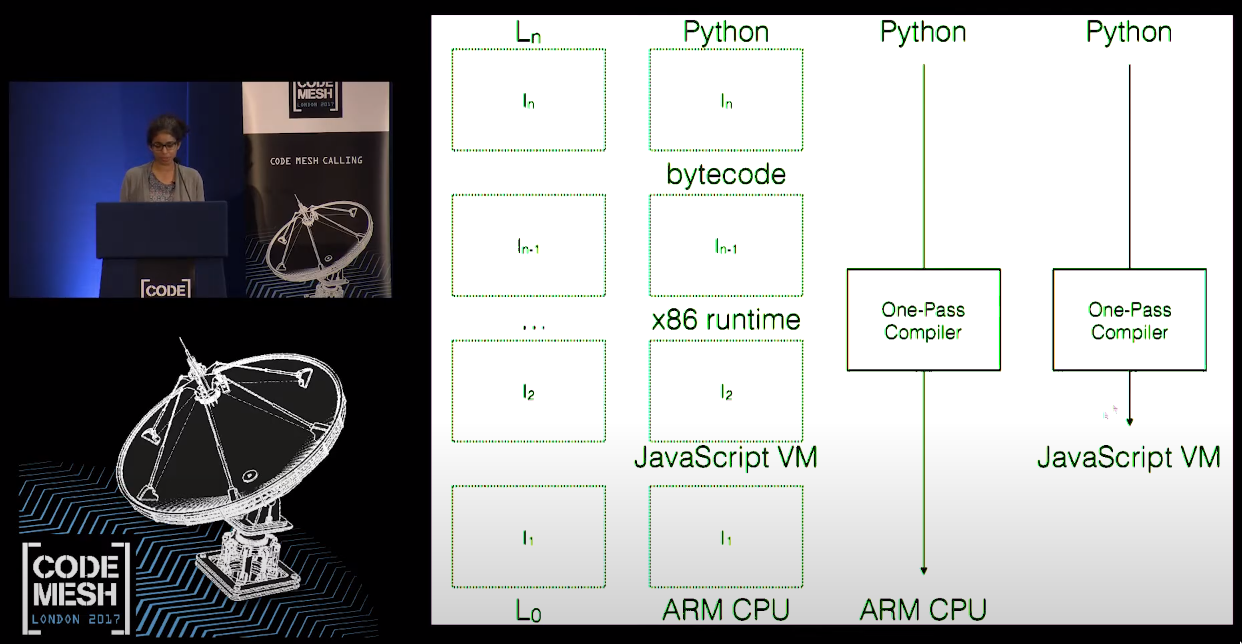
\includegraphics[width=\linewidth]{torres.png}
  \legend{Code Mesh, presentation ``Towers of Interpreters'', by Nada Amin}
\end{figure}

The characteristic problem of concatenate a system of software, one on
top of the other, introduces complexity to maintaining compatibility
among program's versions and it's performance. The study of these
behavior and it's theoretical solutions posses a field of it's
own. And, this field is autonomous, detached, for an example, from
which languages compose the Tower of Interpreters; or which type of
application we are dealing with \cite{amin2017towers}. The object of
study is the final behavior of the system, and if it's a collapsible system. 

\begin{figure}[ht]
  \centering
 \caption{\label{fig:tower2} Categorization of the study of towers of interpreters}
  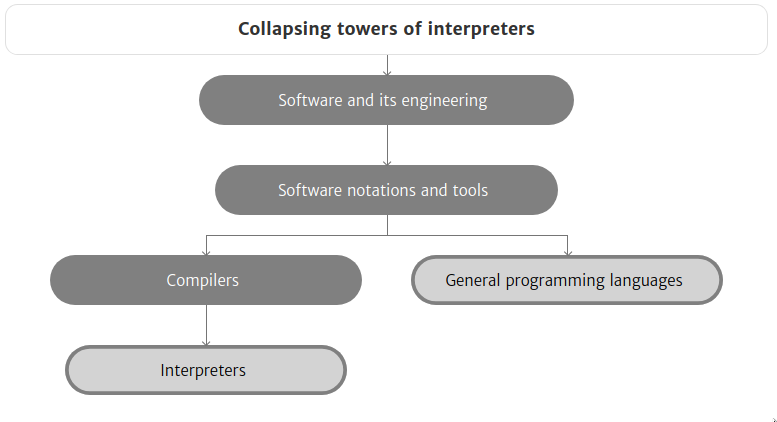
\includegraphics[width=0.5\linewidth]{torres2.png}
  \legend{Reference: \cite{amin2017towers}}
\end{figure}

Finally, the OSes consist in a big tower-collapser of
interpreters. They are subordinate to collapsing firmware, middleware
and high-level software. Therefore, as well as the OS conduct this task,
as much the user-developer experience is facilitated.

\begin{figure}[ht]
  \centering
 \caption{\label{fig:os} Towers of interpreters and the Operational Systems.}
  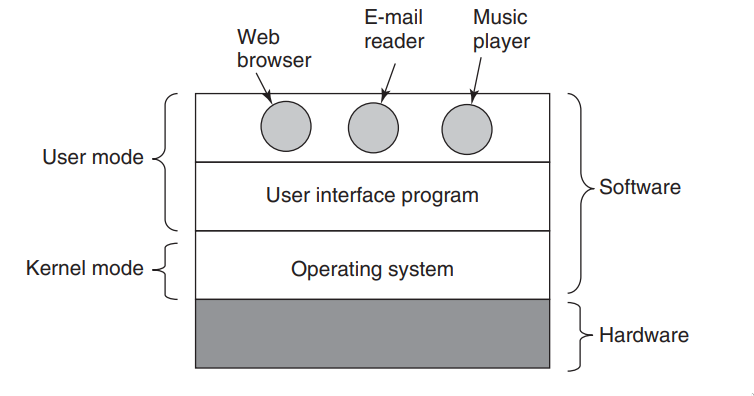
\includegraphics[width=0.5\linewidth]{tower-os.png}
  \legend{Reference: \cite{tanenbaum2015modern}}
\end{figure}

\begin{citacao}
If every application programmer had to understand how all these things work in detail, no code would ever
get written. Furthermore, managing all these components and using them optimally
is an exceedingly challenging job. For this reason, computers are equipped with a
layer of software called the operating system, whose job is to provide
user programs with a better, simpler, cleaner, model of the computer
and to handle managing all the resources just mentioned. \cite{tanenbaum2015modern}
\end{citacao}

\section{On the influence of education in adoption}

In the bibliographical literature, it's clear that the rate of OSS adoption in the Industrial sector - commonly refereed as``Production'' - depends heavily on both: competency and the level of expertise a project require \cite{li2013all,gallego2015open,spinellis2012organizational}.

At the same time, the adoption depends directly on the intrinsic inclination of the Informational Technology (IT) team \cite{racero2021can}. 

Therefore, regardless of how much a professionalizing course may increase the \textit{intensity} and \textit{quickness} of adoption. Data shows that, generally, those students and professionals positively correlated to \textit{seeking autonomy} would adopt it \cite{racero2020predicting}. This means that intrinsic motivation is key \cite{gallego2015open}. Nonetheless, it's important to notice that there exist a net-effect in adoption \cite{spinellis2012organizational}. e.g., how much more peers adopt it, the more likely to any given individual to adopt it.      

\section{Performance and the current trend as reasons for adoption}

Research with different areas of benchmarks state a performance gain, when utilizing GNU/Linux, compared to Windows \cite{sulaiman2021comparison}. Although, even more important, the key benefits are not in the differential performance \textit{per se}, but in the training one naturally goes through upon utilizing a totally community-dependent Operational System. 

Thereof, using GNU/Linux is a door for an individual professional shift. At the same time, this personal use increases the probability of adoption in whichever Industry carrer one may lead \cite{hauge2008adoption}. Combined with that fact, the Industry per se has no observable effect on Open Source development of projects - as so far as measured in 2008 \cite{hauge2008adoption}.

\section{The set-conjunction between physics engineer and FOSS's users}

We note that the deepness of training proposed, in graduation level, for a physics engineer makes them perfect candidates for the use of FOSS. Because, both trainings imply a \textit{a priori} necessity for autonomy and purposeness \cite{schrape2019open,racero2020predicting}; imply a profound and will for generalistic technical knowledge \cite{li2013all,gallego2015open}.

\section{How to leverage the potencial of OSS in Industry and Academia}

In the present work, we utilized of many concept demonstrations, in
which the autor has developed or/and extended applications, in a
context of free and open source. Also, we present how can one
collaborate in the community and how does that collaboration can imply
significant professional connections. This way, both the so called
``soft skills'' and ``hard skills'' benefits have been elucidated, in practice.  

\chapter{Bibliography review}
\section{Open Source}
\label{sec:opensource}

Any program which permits the user-developer to have the following liberties:
\begin{enumerate}
\item The right to run the program, as seen fit, for any end.
\item The right to access the source code and study it.
\item The right to copy and redistribute it.
\item The right to modify the software.
\end{enumerate}

Practically, the Open Source community fundamentally base itself upon
the free distribution of it's tools and programs. One of the differential
advantage of having innumerable other people extending the same
software is that the advancement of the frontier of the program, in
many directions, increases rapidly in relation to a program controlled
by a limited number of programmers.

\subsection{Diversity}
\label{sec:diversity}

Given that one fundamental right of OSS is the modification and
propagation of new modified versions. This right implies in the
observable wide range of maintained versions of these software, which
doesn't have a parallel in any other technological enterprise. 

For an example, one key application in any user's computer is a general
Graphical User Interface (GUI)'s manager, commonly known as Window
Manager (WM). These can be both Floating or Tilling, or mixed WM,
e.g., Floating WM are those that the user must hover windows and
adjust them manually; Tilling WM are those that a pre-defined program
have a set of rules to resize automatically the windows in a screen.

While private Operational Systems (OS), as Windows and MacOS, have
frequent releases - a total of twenty five releases for
Windows. Generally, they've few \textit{active} versions; Windows have
currently four \cite{wikipedia_2021W}. MacOS also have four active
versions \cite{wikipedia_2021Mac}.

The fact there are only narrowly supported versions is due to, among
many contributing factors, users lack the right to alter and extend
the software's behavior. Therefore, they fall victims of discontinued
support and restrictive access to the company's official upgrades. 

On the other hand, there exists, in parallel, around two hundred
seventy eight available distributions of Linux
\cite{wikipedia_2021Linux}. Of which, there are main/root
distributions, which each embody a set of different principles; theoretical and practical philosophies of how to extend software.  

Thus, just as with any other scope of software, the variability of
FOSS always will be grater than monopolized ones.

\section{GNU/Linux}
There are root distributions of Linux, from which many other
distributions emanate. Generically, these partitions are called
families. We cite some of the most influential and popular ones, Red
Hat Linux (\faIcon{redhat}), Debian ({\uni{}}), CentOS
(\faIcon{centos}), Fedora(\faIcon{fedora}), Pacman-based
({\uni{}} /{\uni{}} ), OpenSUSE (\faIcon{suse}),
Gentoo-based ({\uni{}}{} ), Ubuntu-based(\faIcon{ubuntu}),
Slackware ({\uni{}}{} ), Open Sourced-based and the
Independent Distributions ({\uni{}{}}/\faIcon{linux}).

\begin{figure}[!htb]
  \caption{\label{fig:linux-genealogy} Genealogy of Linux's Distributions}
  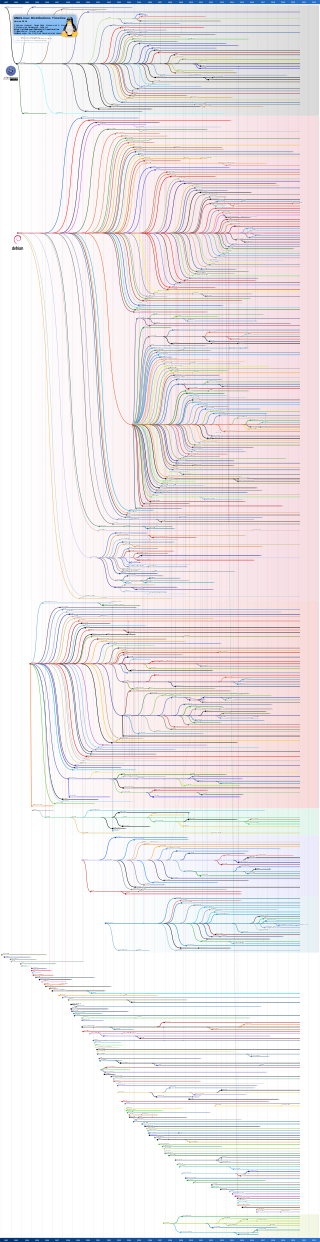
\includegraphics[height=\textwidth, angle=-90]{diversidade}
  \legend{Genealogical history of Linux Distributions \cite{wikipedia_2021Linux}}
\end{figure}


\subsection{\label{sec:linux-origin}Historical Origin}

The GNU/Linux began as two separeted and different directions. GNU
stands for ``GNU's Not Unix'', a recursive name. And GNU initialy has
been developed as a collaboration of revolted academics by the
restrictive secure system of the MIT Lab (Laboratory of Computer
Science - LCS) \cite{stallman2002my,emacswiki2021history}. Amongst
them, there was the still active Richard Stallman, which heavily
worked on the text editor of the time - already ten years into
development. This editor became Emacs \cite{emacswiki2021history}.   

Parallel to these events, Linus Torvalds had been developing an open portatible
operational system, as his master's thesis
\cite{torvalds1997linux}.

Finally, both projects united in a symbiotic system, of which the OS
was Linux (the formentined portible kernel) and the GNU's interface
program whit all utilities one may has had in their computers at the
time \cite{stallman1997}  

\subsection{Emacs}

As has been seen in \href{sec:linux-origin}, the GNU project already
had developed a variety of applications, all of which, incorporated
into Linux. This way, the OS gained a ``body''. The Emacs,
particularly, characterize one of the first software extensively
extended, as a project, in a open community.

Although, the label given to Emacs as an ``editor'' covers it's main
function. Actually, the fundamental role of Emacs equates to
evaluating Elisp expressions. Elisp as in a dialect of
Lisp. Therefore, as an interpreter of a language, it has Turing
complete capabilities. So it has a complete-system capability
\footnote{The GNU/Guix implementation of Linux, has been implemented
  in Scheme - a cousin with better performance than Elisp}.      

Even though Emacs usual use has been of an Integrated Development
System (IDE), by it's unlimited potentiality and expressiveness, there
exists packages and applications written in Elisp to become a fully
featured Window Manager (WM). That is, Emacs, through Emacs's X Window
Manager (EXWM), can serve as a graphical and manager interface to
other applications. 

\begin{figure}[ht]
  \centering
  \caption{\label{fig:exwm1} EXWM - Emacs X Window Manager}
  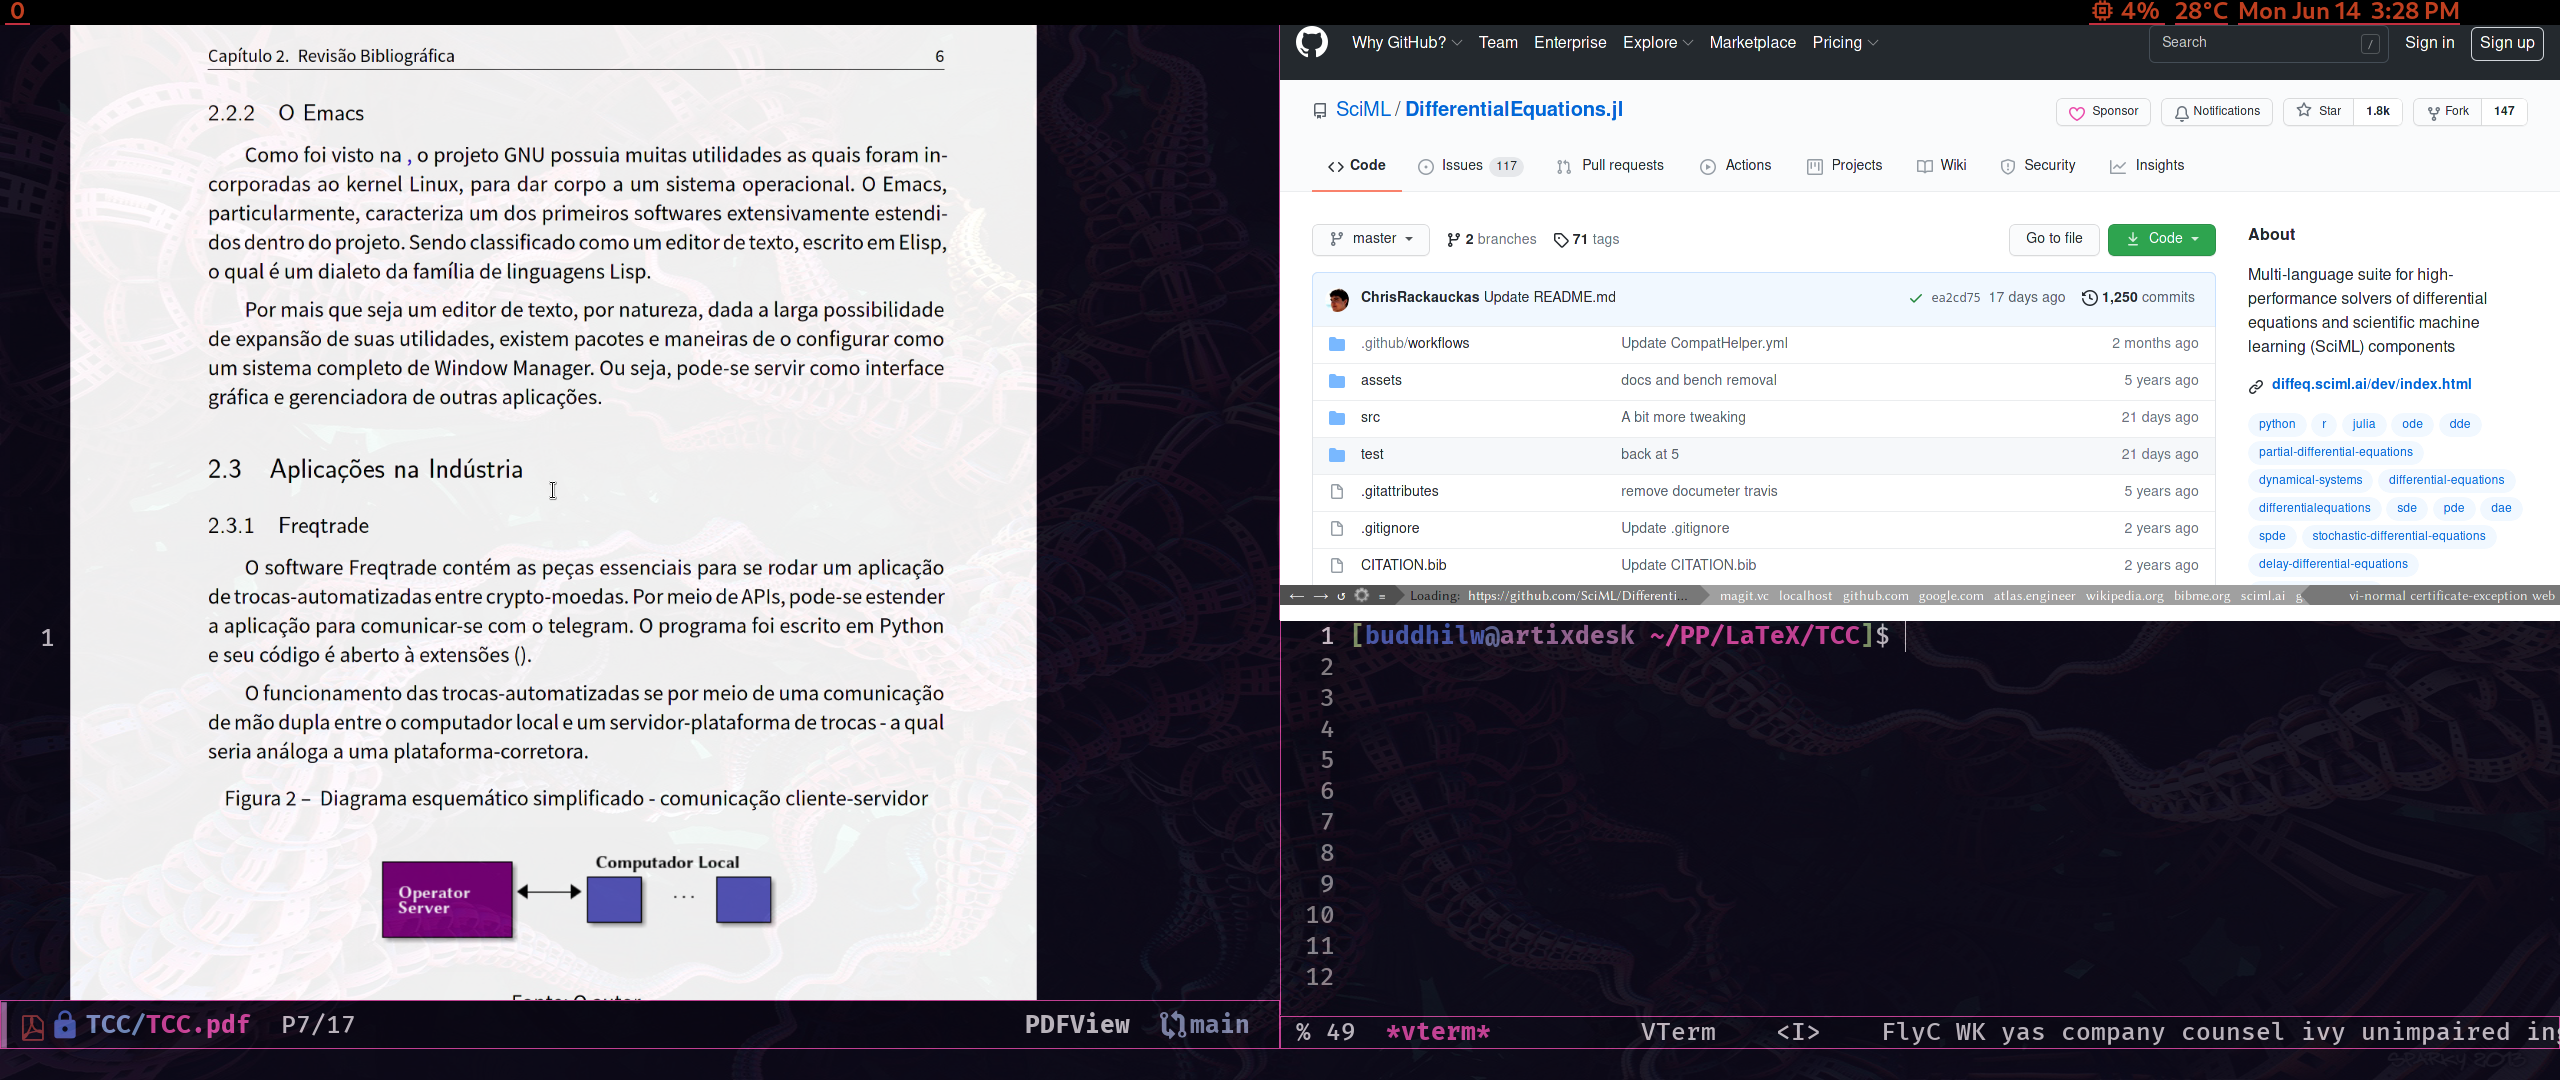
\includegraphics[width=\linewidth]{exwm2.png}
  \legend{Source: author's WM ambient.}
  % \legend{Fonte: foto do ambiente de WM do autor.}
\end{figure}

\autoref{fig:exwm1} exemplifies a desktop environment which can render
images, PDFs, Browsers et el, through Emacs. 

\section{Performance comparison among OS adoption}

\subsection{Performance}
In user-level applications, the efficiency and processing benchmarks
favor Linux over Windows \cite{sulaiman2021comparison}.

In the same hardware, the underground/underlying programs maintaining
a stationary Windows consume around 5\% of CPU and 41\% of RAM. In the
mean time, Linux Mint - a popular distribution of Linux - consumed
1.8\% of CPU and 24\% of RAM. A pronounced difference of more than
200\% in CPU use efficiency and approximately 200\% in RAM efficienty \cite{sulaiman2021comparison}. 

A VBS-program script execution \footnote{An application concerning the
  labeled ``Office'' bundle.} amounts to a difference in
time-execution of 4.249 seconds. In which, Linux
Mint took 0.501 seconds, against a 4.75 seconds for Windows. E.g.,
there exist a roughly $\frac{4,75-0,501}{0,501}= 423\%$ in
time-execution performance \cite{sulaiman2021comparison}.

Lastly, there also exists other researches done with technical rigor in a
broad spectrum of other applications and hardware. To name a few, in
wireless \cite{SDevan2013WINDOWS8V}; parallelism and management of
server applications \cite{aveleda2010performance}; scientific programming (Fast Fourier Transform) et al
\cite{d2011performance}; performance on Virtual Reality (VR)
application \cite{thubaasini2010efficient} etc. All of which present
different kinds of advantages for Linux-use compared to
Windows. Although, against what is expected in view of Industry sector
adoption, Linux has almost no difference, and sometimes can be worst
depending of memory usage of the application \cite{ristov2013}, than Windows performance on
multi-threaded and parallel systems, typically founded in cloud/cluster
server use-case \cite{aveleda2010performance}.

\subsection{FOSS adoption demography}

Fritzgerald enunciated, in 2006, that the adoption profile of users of
Open Source Software (OSS) passed through a phase ``OSS 2.0''. This
phase was characterized as a transcendence from the mentality that the
only people who would be able to use the system would be ``hackers''
\cite{fitzgerald2006transformation}. And, furthermore that such OS
were even becoming ``\textit{mainstream}''. That is, it became a common
place in society and industry. He also professed the hypothesis that
OSS project's activities were significant influenced due to big companies. 

In 2008, another research tried to quantitatively verify the
hypothesis. The data was obtained by questioners and interviews of
Finland software industries. In contrast to the Fritzgerald's
characterization, 50\% of the companies utilized vastly FOSS,
although, they had negligent impact of the development carried by the
community. Lastly, more than 30\% of these companies told that at
least 40\% of their companies value on software was due to services
done by the community \cite{hauge2008adoption}. Also relevant, these
were mostly small to medium size enterprises.    

In 2012, a study on big companies use of OSS - a thousand companies listed on US
Fortune magazine - have derived some conclusions \cite{spinellis2012organizational}: 
\begin{itemize}
\item Adoption is directly related to IT's team need for expertise on
  the work they would partaken, as well as efficient cautiousness \cite{gallego2015open,
 li2013all}.
\item Exponential growth on adoption, once the existence of an
  accumulation of users in the company. 
\item There exist a network effect and the effect is notorious in big companies.  
\end{itemize}

Therefore, adoption in small, medium and big companies process vary,
and there are no salient effects caused by companies on the expansion
of open source projects. Nonetheless, these companies still benefit
from the later \cite{spinellis2012organizational,hauge2008adoption,
  fitzgerald2006transformation}. Still, the most relevant positive-effect on
the OSS and community is due to small enterprises \cite{kshetri2004economics}.  

Regarding the expansion of the FOSS development paradigm and
ecosystem, undoubtedly there is an grow and ubiquity of adoption
\cite{schmidt2016agile}. Moreover, FOSS has been considered in
economical papers as the innovatory cradle of software industry \cite{schrape2019open,schmidt2016agile}.

More recent studies, dating to 2021 and 2020, determine that,
independent of a company size, adoption depends directly on training
of IT and autonomous inclination towards these tools
\cite{racero2020predicting}. Finally, individual adoption and belief
on the effectiveness of these software depend primarily on intrinsic
factors, and is independent of previous training. Even though,
training on OSS notoriously escalates those users inclined for it \cite{racero2021can}.       

\section{Industry Application Demonstration}
\subsection{Freqtrade}
The \emph{Freqtrade} software contains the essential pieces for a
working-application of automated trading of crypto-currencies. By
means of APIs, it's possible to extend the application so to
communicate with the Telegram app. The program has been written in
Python and the code base is open, which rely on one hundred and
forty seven contributors. It's existence dates back to may 2017 \cite{fang2020cryptocurrency}.



The functioning of automated trading goes through a two-way
communication between the local computer and a platform-server of
trading - which would be Angles to a broker.

\begin{figure}[ht]
  \centering
    \caption{\label{fig:diagrama-freqtrade} a simplified schema of
      client-server communication}
  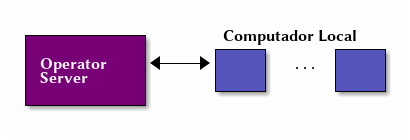
\includegraphics[width=0.6\linewidth]{Imagens/server-client-fq_4.png}
  \legend{Resource: The authors.}
\end{figure}

A great part of the work on writing an automated robot, for any
application end, boils down to programming communication protocols
with server. Because, the robot should be capable of telling the
server which operations should happen, both as means of a response to
the client - e.g., a ``store data on local machine'' request -, as
well as internal operations that should take place on the server -
e.g., execute buy and sell orders on crypto-current exchanges.  

\begin{figure}[ht]
  \centering
    \caption{\label{fig:diagrama-freqtrade2} Schematic representation
      of client-server communication.}
  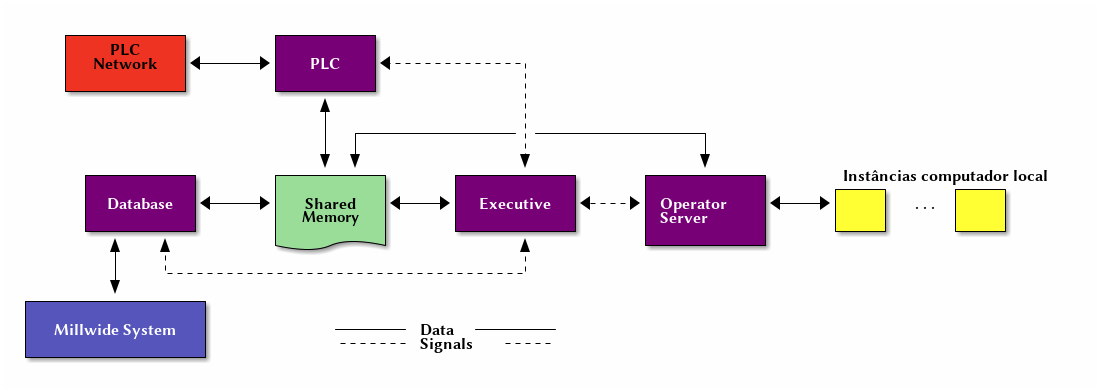
\includegraphics[width=1\linewidth]{ditaa_4.png}
  \legend{Resource: the author.}
\end{figure}

Thus, a schematic representation of this complexity could be seen in \autoref{fig:diagrama-freqtrade2}.

By utilizing OSS, all this complexity
(\autoref{fig:diagrama-freqtrade2}) becomes close to the first schema
(\autoref{fig:diagrama-freqtrade}). Because, all the structural
abstraction has already been dealt of, by this application. To make
use of this advantage, one just need to read and comprehend the
documentation and extend the application to it's use.

\clearpage
\subsection{OR-Tools}
\label{sec:ortools}

\begin{citacao}
Linear Programming is viewed as a revolutionary development giving us
the ability for the first time to state general objectives and to
find, by means of the simplex method, optimal policy decisions for a
broad class of practical decision problems of great complexity. \cite{dantzig1983}
\end{citacao}


The OR-Tools project translates into a series of code libraries
developed in a open sourced manner, initially developed by
Google. Possible ports exist to C++, Python, Java, C\# and .Net.  

The name is given due to Operational Researches Tools acronym, ORT.

We list all category of tools which are under OR-Tools \footnote{https://github.com/google/or-tools},

\begin{enumerate}
\item A constraint programming solver;
\item A linear programming solver;
\item  Wrappers around commercial and other open source solvers, including mixed integer solvers;
\item  Bin packing and knapsack algorithms;
\item  Algorithms for the Traveling Salesman Problem and Vehicle Routing Problem;
\item  Graph algorithms (shortest paths, min cost flow, max flow, linear sum assignment).
\end{enumerate}


The use of this tool can help solve the common problem of
Scheduling. Structurally, this class of algorithms relate to solving
puzzles as Sudoku - for which there are dynamical constraints upon
interaction \cite{simonis2005sudoku}. 

In general, these problem fall under a mathematical and computational
field called Constrained Optimization \cite{bertsekas2014constrained}. 

Not rarely, the typical problem in Constrained Optimization can fall
under a NP-hard problem (a problem for which the Combinatorics of the
system have a exponential ratio, not describable by a polynomial). A
classical example is the ``job shop problem'', for which a seemly
simple and practically ubiquitous task, actually is a NP-hard problem \cite{zhang2019review}.   

Just as in non-deterministic differential equations, or in
differential equations which do not have an analytical solution, it's
common to use numerical solutions. When there one find a NP-hard
problem, analogously, it's used genetic-algorithms and other
reinforced-learning algorithms \cite{zhang2019review}.  

P vs NP problem is one of the open problems in mathematics which has
deep implications to computing. Furthermore, it's listed among the ten
Millennium Prize Problems, of which only one has been solved \cite{cook2006p}.

The Millenium Prize Problems:

\begin{itemize}
  \item Birch and Swinnerton-Dyer conjecture
  \item Hodge conjecture
  \item Navier–Stokes existence and smoothness
  \item P versus NP problem
  \item Poincaré conjecture (solved)
  \item Riemann hypothesis
  \item Yang–Mills existence and mass gap
\end{itemize}



\subsubsection{Application on Economics}

The job scheduling problem thus is central to many areas of
science. For example, generalizing the problem of Operational
Research in economics, we have

\begin{citacao}
The problem of allocating scarce resources among competing ends is
central to economic analysis.

(...) The problem of optimal allocation of scarce resources can thus
be summarized as the optimization of some objective(s) subject to
constraints. \cite{luptacik2010mathematical}
\end{citacao}

Which means that this field has great application for tools as OR-Tools.

\begin{citacao}
The emphasis is given to the exposition of mathematical optimization as an
instrument for qualitative analysis and to a wide range of
applications in economics, including efficiency analysis, industrial
economics (with focus on regulatory economics), international
economics, input–output economics, quantitative economic policy and
environmental economics. \cite{luptacik2010mathematical}
\end{citacao}

\subsubsection{Application to environmental policies}
Policies annually are pitched by Intergovernmental Panel on Climate
Change (IPCC) on how business should constrain their business matrix
of energy etc, so to meet environmental goals
\cite{keysser20211}.

There is an open field to transform these
measures into actionable plans to enterprises. If sufficiently
quantitative, such measures could be incorporated in programs is
Operational Researches software \cite{luptacik2010mathematical}.

There are some papers which gives Optimization Models for
air pollution control \cite{abrams1975optimization}, countries comparative
eco-efficiency \cite{dyckhoff2001measuring} etc. We cite a quotation
from ``Eco-efficiency analysis of industrial system in China: A data
envelopment analysis approach'' \cite{zhang2008eco}.

\begin{citacao}
 In this connection, strategies for optimizing the use of resources or
environment as expressed in more efficient way play a
particularly important role. Eco-efficiency, which is an instrument for sustainability analysis, indicating an empirical
relation in economic activities between environmental cost
or value and environmental impact, has been proposed as a
route to promote such a transformation \cite{mickwitz2006regional}.
\end{citacao}

And we can see that this is the case-use, at least in quantitative
researches in ecology; we look into one result from US eco-efficiency research on a decade of data,

\begin{citacao}
 Although an increase in both the mean RR (0.3–0.4) and the mean E-RR
 (0.38–0.52) scores was recorded from 1995 to 2014, this was concluded
 to be unsatisfactory, since the majority of the industries’
 eco-efficiency results were still below 0.5. \cite{ezici2020assessing}
\end{citacao}

And, the conclusion is that,

\begin{citacao}
The findings of this study suggest that substantial policy changes are
required immediately to shift the negative trend in renewable energy
use to comply with UN Sustainability Development Goals 7 and 13. \cite{ezici2020assessing}
\end{citacao}



We also emphasize, that this problem can seem unrelated to other
things like grammar analysis on authorship, or ecological policies
formulation. But, indeed they are related. 

Research using eco-efficient measures upon constrains for making
policies has matured. And plans utilizing it as an constrain can be
pathways to saving the world from ecological decimation.

\begin{citacao}
Urban-industrial symbiosis (UIS) is an important system innovation via
sectors integration, and has been widely recognized as a novel pathway
for achieving regional eco-industrial development. Eco-efficiency, as
a mature approach and indicator, offers an effective tool to uncover
both the status and trends of such a transformation \cite{bian2020sectoral}.
\end{citacao}

\subsubsection{Application to other areas}

The areas that such optimization constrains are applied are
uncountable. We cite some not so intuitive areas:

\begin{itemize}
\item Natural Language analysis and evolution \cite{potts2010harmonic,
  heinz2018computational}
\item Plans to maintain production of rural areas in Brazil, with no
  need for further deforestation \cite{costa2018socio}.
\item Planning upon corporate social performance
  \cite{chen2011measuring,jacobs2016operational}.
\item Public transportation \cite{schiewe2020integrated} 
\item Traffic Control \cite{delle2019feedback}
\end{itemize}

\section{Demonstration in Academic Applications}

% \clearpage
\subsection{DifferentialEquations.jl}

The numerical library, DifferentialEquations, has one of the best
performances among numerical software
\cite{rackauckas2017differentialequations}. The performance is
comparable to implementations in FORTRAN and C. Also, this library has
many ports \footnote{Capability to interoperate besides the language it
was written in.}, some of the languages in which you can use it are in Python, R and Julia itself.

Among the many different category of problems this library can deal
with are \cite{rackauckas2019confederated,rackauckas2017adaptive,rackauckas_stability-optimized_2018,sykora2020stochasticdelaydiffeq,rackauckas2018comparison,rackauckas2019diffeqflux,rackauckas2020universal,gowda2019sparsity,ma2021modelingtoolkit},

\begin{itemize}
\item Discrete equations (function maps, discrete stochastic (Gillespie/Markov) simulations)
\item Ordinary differential equations (ODEs)
\item Split and Partitioned ODEs (Symplectic integrators, IMEX Methods)
\item Stochastic ordinary differential equations (SODEs or SDEs)
\item Stochastic differential-algebraic equations (SDAEs)
\item Random differential equations (RODEs or RDEs)
\item Differential algebraic equations (DAEs)
\item Delay differential equations (DDEs)
\item Neutral, retarded, and algebraic delay differential equations (NDDEs, RDDEs, and DDAEs)
\item Stochastic delay differential equations (SDDEs)
\item Experimental support for stochastic neutral, retarded, and algebraic delay differential equations (SNDDEs, SRDDEs, and SDDAEs)
\item Mixed discrete and continuous equations (Hybrid Equations, Jump Diffusions)
\item (Stochastic) partial differential equations ((S)PDEs) (with both finite difference and finite element methods)
\end{itemize}

\subsubsection{Julia portability}

The steps to use the library in Julia are,

\begin{verbatim}
# Using the package Pkg, so to manage packages. 
using Pkg
# Add and/or download the DifferentialEquations.jl package in the project 
Pkg.add("DifferentialEquations")
# Access all the functions defined in the package 
using DifferentialEquations
\end{verbatim}

\subsubsection{Python portability}

In a terminal using the package manager \textit{pip},
\begin{verbatim}
pip install diffeqpy
\end{verbatim}

In a terminal, running the Python interpreter,
\begin{verbatim}
>>> import diffeqpy
>>> diffeqpy.install()
\end{verbatim}

An optional step is to add numba, so to optimize the code performance,
\begin{verbatim}
pip install numba
\end{verbatim}

Finally, import the package in a file and use in a program.
\begin{verbatim}
import diffeqpy
\end{verbatim}

\subsubsection{R portability}

To install, use
\begin{verbatim}
install.packages("diffeqr")
\end{verbatim}

% Na primeira chamada de,
In a first call,
\begin{verbatim}
diffeqr::diffeq_setup()
\end{verbatim}

This way, the package will be downloaded, directly from
DifferentialEquations.jl. An alternative is to use
\href{https://cran.r-project.org/web/packages/diffeqr/index.html}{the
  CRAN maintained subset}.
% Será feito o download do DifferentialEquations.jl. Um subconjunto específico do pacote é ativamente mantido \href{https://cran.r-project.org/web/packages/diffeqr/index.html}{no CRAN}.

\subsection{\LaTeX}

The \LaTeX{} has fundamentally differentiate the many tasks in the
typography of a document. The language permits a separation of
formatting-tasks, and the content-writing. This way, the user can
focus exclusively on content, in a fundamental step in document
writing. And in another moment, focus solemnly on format and
aesthetics.
% O \LaTeX{} possui separação entra as tarefas de produção de um
% documento. A linguagem permite-nos separar as tarefas de formatação do texto, da escrita de seu conteúdo. Desta forma, o usuário concentra-se
% exclusivamente em seu conteúdo, em um estágio da escrita do documento. E, na formatação de sua aparência, em outro momento.

Therefore, there a quality gain in production. Just as one is rewarded
with the total control of the document, because every graphical
disposition and behavior is defined by open code. Furthermore, one can
extend already written templates and packages which do usual
formatting. The typographical system in \LaTeX{} has been considered,
also, one of the most sophisticated software of it's category, mostly
because of this bottom-up paradigm one naturally uses \cite{haralambous2007}.
% Assim, ganha-se em qualidade de produção. Bem como, ganha total autonomia sob o documento, pois a programação da disposição gráfica dos elementos textuais pode ser programada - isto é, modificada indefinidamente, a partir dos comportamentos padrões dos pacotes utilizados. O sistema tipográfico de \LaTeX{} chegou a ser considerado o sistema digital de
% tipografia mais sofisticado que existe, devido a essa paradigma de
% programação funcional, \textit{bottom-up} \cite{haralambous2007}.

The \LaTeX{}, technically, is the union between the typographical
language \TeX{}, invented by Donald Knuth, for high quality documents
\cite{knuth1986}. And, the powerful macro ecosystem, which extend the \TeX{}
programming, for which we call \LaTeX{}.

Initially \LaTeX was developed by Leslie Lamport, with his personal
use-case formatting programs \cite{lamport1994}. Thus, \LaTeX{} is not
just a language, but a conjunction of macros and standard
environments, which is actively maintained, modified, and extended by
the open community.
% O \LaTeX, tecnicamente, é a junção do sistema de tipografia \TeX,
% inventado por Donald Knuth, para tipografia de alto nível
% \cite{knuth1986}; com os poderosos macros que facilitam a extensão do programa \TeX, a qual damos o nome de
% \LaTeX. O \LaTeX{} foi inicialmente desenvolvido por Leslie Lamport, com
% seus pacotes fundamentais de formatação \cite{lamport1994}. O \LaTeX,
% por conseguinte, não é somente uma linguagem de tipografia de alto
% nível, mas também um conjunto de macros para facilitar a tipografia em
% si. Qualifica-se, assim, como um sistema de preparação de documentos;
% uma linguagem markup de domínio específico.

\subsubsection{The canonical ABNT class for scientific production}

What is called as canonical are a set of documents following the more
general and robust ABNT (Associação Brasileira de Normas Técnicas)
norms. These canonical forms exist for scientific articles, technical
reports, academic works as thesis, dissertations and research
projects, books and presentations \cite{abntex2012}. 
% Documentos sob os requisitos das normas ABNT (Associação Brasileira de Normas
% Técnicas) para elaboração de documentos técnicos e científicos
% brasileiros - como artigos científicos, relatórios técnicos, trabalhos
% acadêmicos, como teses, dissertações, projetos de pesquisa e outros
% documentos do gênero \cite{abntex2012} - é ao que se chama classe
% canônica ABNT.

\begin{citacao}
  Os documentos indicados tratam-se de “Modelos Canônicos”, ou seja,
  de modelos que não são específicos a nenhuma universidade ou instituição, mas
  que implementam exclusivamente os requisitos das normas da ABNT, Associação
  Brasileira de Normas Técnicas. \cite[Cap. 1]{araujoclasse}
\end{citacao}

% % \clearpage

% As normas as quais prescrevem o modelo canônico são:
The norms prescribed by the canonical model are:

\begin{itemize}
\item \textbf{ABNT NBR 6022:2018:} Informação e documentação -
  Artigo em publicação periódica científica - Apresentação.
\item \textbf{ABNT NBR 6023:2002:} Informação e documentação -
  Referência - Elaboração.
\item \textbf{ABNT NBR 6024:2012:} Informação e documentação -
  Numeração progressiva das secções de um documento - Apresentação.
\item \textbf{ABNT NBR 6027:2012:} Informação e documentação -
  Sumário - Apresentação.
\item \textbf{ABNT NBR 6028:2003:} Informação e documentação -
  Resumo - Apresentação.
\item \textbf{ABNT NBR 6029:2006:} Informação e documentação -
  Livros e folhetos - Apresentação.
\item \textbf{ABNT NBR 6034:2004:} Informação e documentação -
  Índice - Apresentação.
\item \textbf{ABNT NBR 10520:2002:} Informação e documentação -
  Citações.
\item \textbf{ABNT NBR 10719:2015:} Informação e documentação -
  Relatórios técnicos e/ou científico - Apresentação.
\item \textbf{ABNT NBR 14724:2011:} Informação e documentação -
  Trabalhos acadêmicos - Apresentação.
\item \textbf{ABNT NBR 15287:2011:} Informação e documentação -
  Projeto de pesquisa - Apresentação.
\end{itemize}

\section{Canonical works on Scientific Computer Science}
\label{sec:scim}
% \section{Trabalhos Canônicos na Área de Computação}
\subsection{Structure and Interpretation of Classical Mechanics (SCIM)}
\label{sec:scim}
The scientific library of classical mechanics, written in Scheme (a
Lisp dialect), has been used to teach master's degree MIT
students. Accompanied to the library there is the book, which servers
as didactic material for the course \cite{sussman2015structure}.
% A bilioteca científica de simulações de mecânica clássica, em Scheme
% (um dialeto de Lisp), foi escrito com intento de ser utilizado em
% cursos de mestrado no MIT. Acompanhado à biblioteca, existe o livro,
% o qual serve de material didáctico ao curso
% \cite{sussman2015structure}.

The library and the book are open sourced.

\subsection{Structure and interpretation of computer programs (SICP)}
The scheme course (SICP), which is teach as the foundations of
computer science course on MIT, has accompanied as textbook one of the
most world wide recognized books in computer history
\cite{abelson1996structure}.

This course has been the pioneer on givin emphasis to the
epistemological activity, when programming. The use of Scheme, which
has a uniform notation (only one form), was revolutionary. This has
shown to work well, instead of presenting the trending language
in Industry, in a given moment - which is the standard approach.  
% O curso de Scheme (SICP), o qual é ensinado como materia básica de computação no MIT, possui como acompanhantes um dos mais influentes livros já escritos na história da computação \cite{abelson1996structure}. O curso é pioneiro em aprofundar-se epistemologia da programação. Onde, o uso de Scheme, o qual possui notação uniforme para todas as funcionalidades da língua foi revolucionário. Conquanto, em contraste aos outros cursos de fundamentos da computação focavam em ensinar a linguagem mais amplamente utilizada no momento.

The SCIM (\autoref{sec:scim}) course as a predecessor to SICP. The course and
the text book still are in use in MIT and a number of other
universities around the world. A non-exaustive list can be found at
\url{https://mitpress.mit.edu/sites/default/files/sicp/adopt-list.html}. At
least twenty universities adopts, distributed in more than eight countries.
% O curso SCIM (\autoref{sec:scim}) foi um precursor de SICP. O curso
% continua ativo e o livro continua a ser utilizado amplamente no MIT,
% e em inúmeras outras faculdades. Uma lista não exaustiva pode ser
% encontrada em
% \url{https://mitpress.mit.edu/sites/default/files/sicp/adopt-list.html}, em que pelo menos, vinte universidades o adotam, em mais de oito países.

These materials, textbook and the MIT classes, are both free and open
sourced.
\subsection{SCIMUtils - (SCIM) Portability in Clojure}
\label{sec:scimutils}

These are dedicated libraries for rewriting the SCIM programs in
Clojure, which ports many functionalities mentioned in the scientific
library SCIM\note{The library and the course's programs are not the
  same thing} \cite{sicmutils2016github}. This library, therefore, has
been ported to Clojure, which is the most industry-used Lisp
modern-dialect. For example, Nubank bought Cognitect which was the
first and most successful application written in Clojure \cite{clojure2020}. 
% Existe uma biblioteca reescrita em clojure, a qual porta as funcionalidades descritas na biblioteca científica SCIM \cite{sicmutils2016github}. Essa biblioteca é escrita numa das mais modernas linguages de computação com adoção amplamente da Industria, Clojure. Recentemente, a maior empresa utilizado de Clojure até então, a Cognitect, a qual inventou a língua foi comparada pelo Nubank \cite{clojure2020}.

The language has a double quality in it's program. Due to the language
supporting multiple definitions of a function under a name
(polymorphism), it's possible to very easily switch and integrate
numerical and symbolical computations.

Changing inputs one would has one or the other output, by inference
of the Clojure compiler. This is particularly interesting when
solving, for example, Lagrange equations of motion. One can has both
the symbolical results outputted in \TeX{}, and by a change in inputs,
in the same procedure, have numerical data which can be used to
simulate the behavior of physical systems. 


\chapter{Materials and Methods}
% \chapter{Materiais e Métodos}
% O planejamento da monografia seguiu as seguintes etapas:
The planning of the monograph has followed the steps:

\begin{enumerate}
  % \item Contato e estratégias com o orientador;
  \item Contact and develop strategies with the supervisor;
    % \item Determinação do tópico principal; 
  \item Deliniating the main theme;
    % \item Delineação específica dos subtópicos;
  \item Given the date constrains, schedule an fitting agenda;
    % \item Organização da agenda à partir das datas finais objetivadas;
  \item Outline the structure of the TCC;
    % \item Início à escrita do TCC;
  \item Gather of exploratory notes about the topic;
    % \item Junção de notas exploratórias sobre o tópico;
  \item Biliographical reseach;
    % \item Pesquisa bibliografia;
  \item Writting each dedicated topic;
    % \item Escrita de todos os tópicos da monografia;
  \item Reuse past knowledge and use personal practical examples; 
  \item Continuous revision, for each step of the monograph;
    % \item Revisão contínua à cada etapa da monografia;
  \item Organize the presentation;
    % \item Organização de apresentação;
\end{enumerate}

\section{Initial Strategy}
The first steps taken were to determine what would be the best match of student-advisor, based on mutual interest on the topic. Then, began the first general schema of the work, and the schedules.
% Procurou-se um docente tanto familiar ao autor, quanto versado e
% interessado no tópico de pesquisa.

% \section{Delineação do tema}
\section{Theme delineation}
Given that the theme OSS on Industry and Academia has indefinetly many
branches to discuss, we urged to narrow down the boudaries of the
topic to those applications of most famility to the student.
% Dado que o tema softwares livres na indústria e academia é um tópico
% indefinidamente abrangente, houve uma necessidade imprescindível de
% delimitar graduamente o tópico.

In the continuous reviews, we further narrowed the topic by wheigthing
if deepening the analyses wouldn't deviate from the main topics.
% Nas revisões contínuas, determinava-se o quão profundo tinha se
% abordado os tópicos, e se era necessário dar procedência, ou seguir o
% andamento de outras parte da agenda.

\section{Cronological Schedule}
% \section{Organização cronológica}

We followed the Gantt diagram method to orient ourselves, which is a
visual aid to help on following deadlines. At the same time, the
diagram helps to situate oneself in relation to what should the team
be doing.
% Decidiu-se por seguir o método de diagrama de Gantt, amplamente
% utilizado em organização de projetos. As partições temporais foram
% ponderadas pelas datas limites objetivadas.

\section{The monograph theme}
% \section{As fases da escrita da Monografia}

As this monograph mainly falls under an Exploratory Analysis, the main
focus was the theme's literature. We show programs developed by the
open community. 
% Como a monografia se caracteriza como uma Análise Exploratória, o
% enfoque foi na literatura concernente ao Tema.

% <come back> , from OS, WM, to particular applications

On the Academic Application's branch, the emphasis was given to
auxiliary software for research. Also, we shown some software that may
as well be used for teaching physical concepts. 
% Na subtópico acadêmico, procurou-se dar enfoque ambos softwares auxiliares
% de pesquisas, quanto úteis à sala de aula. Bem como, pretendia-se
% explicar conceitos-chave na compreensão da dinâmica histórica e atual
% do ecossistema em que se desenvolve e aplicam softwares.

In the short experience of the student on Industry, we found examples
of software he already made use of.
% Ademais, nas aplicações tecnológicas, o autor documentou softwares que
% já utilizou em situações reais.

\section{Gathering various notes}
% \section{Junção de notas}

One of the open sourced software of most use to the student is
org-mode. In \textit{.org} files, one can take notes, just as in note
applications found in any device. A lot of material was gathered from
those notes to compose the results.
% Ao se utilizar os softwares os autores havia produzido anotações sobre
% o desenvolvimento do software. Uma auto-documentação, enquanto se
% desenvolvia, ou se estudava os mecanismos de uma aplicação. Assim,
% utilizou-se dessas notas para construção da monografia.

\section{Bibliographical Research}
The bibliographical review intended to facilitate the comprehension of
Software Industry. We gathered some cuts of the history of
FOSS. Furthermore, we brought information about some open software
which are considered state of the art, or iconic, on their field of application.
% A revisão da bibliografia objetiva facilitar o entendimento da
% indústria dos softwares, a qual é difere em seu aspecto
% majoritariamente livre e aberto. Além do mais, procurou-se fazer um
% recorte de história, usos e desenvolvimento em estado da arte de
% diversos softwares icônicos.

Most of the historical content about the FOSS movement and software in
general can be found in websites. Particularly, GNU was the main
source of FOSS history. In contrast, most sources on software
development and comparative functionality was found on scientific articles.
% A maior quantidade de informações históricas encontra-se armazenada
% digitalmente, em sites de instituições internacionais, como o
% GNU. Conquanto, nas aplicações procurou-se o embasamento em artigos
% científicos.

We used Google Scholar and Association for Computing Machinery's (ACM)
platform. The student had access due to being a member to the research
engine and papers they have. The content of ACM is mainly about
software and theoretical computation in general. 
% Utilizou-se do Google Scholar e a plataforma da ACM (Association for
% Computing Machinery), da qual o autor é
% membro e na qual existe material especializado em computação e softwares.

\section{Continuous Review}
A fundamental part of the research's organization conciseness was due
to the frequent interaction between the student and the advisor.
% Parte fundamental da organização da monografia foi a troca de
% informações, auxílio, e integração constante das considerações do
% orientador Dr. Wei-Liang.

\section{Presentation Organization}
% \section{Organização da apresentação}
The use of visual software coupled with org-mode \footnote{There are
  dedicated packages in Emacs to make presentations with org-mode
  files https://github.com/howardabrams/demo-it} makes an presentation
interactive. So, much of the work done in the monograph was reused for presentation.
% Na apresentação, procura-se utilizar ferramentas interativas e
% demonstração de conceitos por meio de programação em tempo real
% aplicações. Escolheu-se utilizar da ferramento Org-mode, integral ao
% Emacs.

\chapter{Results and Discussion}
% \chapter{Resultado e Discussões}

\section{Advisor expertise and the theme}
% \section{Convite ao orientador}

One of the applications the student supposed could be done with OSS
was with Lagrangians. SCIMUtils (\autoref{sec:scimutils}) exist in
Clojure - the port of the famous work SCIM. and the advisor had given
lectures on the subject of Classical Mechanics on the university
courses. At the same time, the advisor itself is an user-developer,
using Linux. So, the themes and expertise matched.
% % O autor já havia interagido com o Dr. Wei-Liang, o qual no passado
% havia pedido, a titulo de pesquisarem juntos, que se instalasse o
% sistema operacional do Linux. Ademais, uma das aplicações era na
% resolução e simulação de sistemas resolvidos por Lagrangeanas - tópico
% lecionado pelo orientador, na disciplina de Mecânica Clássica.

% Assim, fortunamente o orientador se sentiu inclinado a participar
% desse trabalho. E, concorda que o ensino sobre a iniciativa Open
% Source, bem como os softwares em si, são detrimentais na vida acadêmica.

\section{Theme delineation}
% \section{Delineação do tema}
The GNU and the OSS initiative have indefinitely many subjects that
could be tackled. There are virtually FOSS written for application on
any human enterprise.   
% A iniciativa GNU e o open source é indefinidamente abrangente. Existem
% softwares abertos escritos para virtualmente qualquer outra área do
% exercício cognitivo do ser humano.

We opted to work on applications most familiar to the student. Also,
we the work focused on presenting the most significant aspects of
FOSS, in geral, for Academia and Industry.
% Necessitou contentar-se em parcialmente mostrar aplicações mais em
% mão, as quais seriam mais relevantes ao escopo da monografia. Bem
% como, optou-se por aprofundar-se em tópicos já utilizados na vida do
% autor para se resolver problemas na academia e na indústria.

Thus, the delimitation on showing the framework for an working FOSS
OS. The delimitation to the OR-Tools and Freqtrade in
Industry. Finally, the use of Clojure, Julia, Python and R as means to
present graphical and numerical applications to abstract ideas in mathematics.
% Assim, a delimitação principal se deu entorno de ferramentas abertas
% das quais, na indústria foram apresentados OR-Tools e
% Freqtrade.

% \subsection{Da Indústria}
\subsection{Industry Applications}

\subsubsection{OR-Tools}
The language used to write this application is C++ \footnote{https://github.com/google/or-tools}. But,
there are ports to Python, Java (thus, Clojure), .Net. All languages
have this program licensed in \textit{copy-left} terms.
% As línguas utilizadas para o desenvolvimento desses softwares foram
% Python e C++. Porém, no caso de OR-Tools existe portabilidade para
% C++ (nativo), Python, Java, .NET. Todos os projetos e línguas possuem licença aberta.

OR-Tools has been designed to tackle conspicuous problems: one of them,
scheduling. Virtually any social-economic enterprise use scheduling in
some moment.

\paragraph{Scheduling work shifts problem}
We offer an example in the following setting. A hospital needs to create a schedule for four nurses over a three-day period, subject to the following conditions:

\begin{enumerate}
\item Each day is divided into three 8-hour shifts.
\item Every day, each shift is assigned to a single nurse, and no
  nurse works more than one shift.
\item Each nurse is assigned to at least two shifts during the
  three-day period.
\item There are 10 nurses.
\item There are 7 days of work.
\end{enumerate}
% OR-Tools destina-se a resolver um problema virtualmente
% conspícuo a qualquer negócio ou estrutura social prestadora de
% serviço. Pois, o problema de agendamento de horários, com condições de
% restrições impostas, é extremamente comum. Por exemplo, para organizar
% turnos de funcionários, em uma empresa; turnos de enfermeiros em um
% hospital - exemplo dado na própria documentação do software etc.

In this problem, the program would translate to \footnote{This problem
is a variation from the one on the project's documentation, https://developers.google.com/optimization/scheduling/employee_scheduling},
% <\lstset{language=python}
Importing the OR-Tools utilities,

\begin{python}
  from ortools.sat.python import cp_model
\end{python}

Stating the constants, and standard input/output functions,

\begin{python}
class NursesPartialSolutionPrinter(cp_model.CpSolverSolutionCallback):
    """Print intermediate solutions."""

    def __init__(self, shifts, num_nurses, num_days, num_shifts, sols):
        cp_model.CpSolverSolutionCallback.__init__(self)
        self._shifts = shifts
        self._num_nurses = num_nurses
        self._num_days = num_days
        self._num_shifts = num_shifts
        self._solutions = set(sols)
        self._solution_count = 0

    def on_solution_callback(self):
        if self._solution_count in self._solutions:
            print('Solution %i' % self._solution_count)
            for d in range(self._num_days):
                print('Day %i' % d)
                for n in range(self._num_nurses):
                    is_working = False
                    for s in range(self._num_shifts):
                        if self.Value(self._shifts[(n, d, s)]):
                            is_working = True
                            print('  Nurse %i works shift %i' % (n, s))
                    if not is_working:
                        print('  Nurse {} does not work'.format(n))
            print()
        self._solution_count += 1

    def solution_count(self):
        return self._solution_count
\end{python}

Giving fixed values to the program,

\begin{python}
def main():
    # Data.
    num_nurses = 10
    num_shifts = 3
    num_days = 7
    all_nurses = range(num_nurses)
    all_shifts = range(num_shifts)
    all_days = range(num_days)
\end{python}

Creating the model constraints,

\begin{python}
    # Creates the model.
    model = cp_model.CpModel()

    # Creates shift variables.
    # shifts[(n, d, s)]: nurse 'n' works shift 's' on day 'd'.
    shifts = {}
    for n in all_nurses:
        for d in all_days:
            for s in all_shifts:
                shifts[(n, d,
                        s)] = model.NewBoolVar('shift_n%id%is%i' % (n, d, s))

    # Each shift is assigned to exactly one nurse in the schedule period.
    for d in all_days:
        for s in all_shifts:
            model.Add(sum(shifts[(n, d, s)] for n in all_nurses) == 1)

    # Each nurse works at most one shift per day.
    for n in all_nurses:
        for d in all_days:
            model.Add(sum(shifts[(n, d, s)] for s in all_shifts) <= 1)

    # Try to distribute the shifts evenly, so that each nurse works
    # min_shifts_per_nurse shifts. If this is not possible, because the total
    # number of shifts is not divisible by the number of nurses, some nurses will
    # be assigned one more shift.
    min_shifts_per_nurse = (num_shifts * num_days) // num_nurses
    if num_shifts * num_days % num_nurses == 0:
        max_shifts_per_nurse = min_shifts_per_nurse
    else:
        max_shifts_per_nurse = min_shifts_per_nurse + 1
    for n in all_nurses:
        num_shifts_worked = 0
        for d in all_days:
            for s in all_shifts:
                num_shifts_worked += shifts[(n, d, s)]
        model.Add(min_shifts_per_nurse <= num_shifts_worked)
        model.Add(num_shifts_worked <= max_shifts_per_nurse)
\end{python}

Call the cp_model to transform the constrains in a solvable format,

\begin{python}
    # Creates the solver and solve.
    solver = cp_model.CpSolver()
    solver.parameters.linearization_level = 0
\end{python}

Finally, print a few of the solutions (5) and give some feedback on
performance and analytics of the problem.

\begin{python}
    # Display the first five solutions.
    a_few_solutions = range(5)
    solution_printer = NursesPartialSolutionPrinter(shifts, num_nurses,
                                                    num_days, num_shifts,
                                                    a_few_solutions)
    solver.SearchForAllSolutions(model, solution_printer)

    # Statistics.
    print()
    print('Statistics')
    print('  - conflicts       : %i' % solver.NumConflicts())
    print('  - branches        : %i' % solver.NumBranches())
    print('  - wall time       : %f s' % solver.WallTime())
    print('  - solutions found : %i' % solution_printer.solution_count())

if __name__ == '__main__':
    main()
\end{python}

The result:
% <\lstset{language=python}
\begin{python}
Solution 4
Day 0
  Nurse 0 does not work
  Nurse 1 does not work
  Nurse 2 does not work
  Nurse 3 does not work
  Nurse 4 does not work
  Nurse 5 does not work
  Nurse 6 does not work
  Nurse 7 works shift 0
  Nurse 8 works shift 1
  Nurse 9 works shift 2
Day 1
  Nurse 0 does not work
  Nurse 1 does not work
  Nurse 2 does not work
  Nurse 3 does not work
  Nurse 4 does not work
  Nurse 5 does not work
  Nurse 6 does not work
  Nurse 7 works shift 2
  Nurse 8 works shift 1
  Nurse 9 works shift 0
(...)
Day 6
  Nurse 0 works shift 1
  Nurse 1 works shift 0
  Nurse 2 works shift 2
  Nurse 3 does not work
  Nurse 4 does not work
  Nurse 5 does not work
  Nurse 6 does not work
  Nurse 7 does not work
  Nurse 8 does not work
  Nurse 9 does not work

Statistics
  - conflicts       : 3540
  - branches        : 67968438
  - wall time       : 102.701620 s
  - solutions found : 561425
\end{python}

When there are too many solutions to a constrain problem, that means
there are too much resources to the given constrain. That is, the
hospital could operate with less workers \footnote{We stopped the
  program before it found all solutions.}. Let's use 3 nurses, keeping
the other constrains.

This gives us, on termination,
% <\lstset{language=python}
\begin{python}
Statistics
  - conflicts       : 386
  - branches        : 2683080
  - wall time       : 15.481512 s
  - solutions found : 279936
\end{python}

But, if we then change the constrains to number of shifts being 4 -
that is, 6 hour-work.

% <\lstset{language=python}
\begin{python}
Statistics
  - conflicts       : 10
  - branches        : 194
  - wall time       : 0.002517 s
  - solutions found : 0
\end{python}
Of course, because one of the nurses would need to work more than once
a day. This would break one of our constrained-condition. We note, though, that there is no continuity in-between the possibility of no solution and the most optimized one. 

Furthermore, the solutions have exponential growth on the \textbf{event space}. Thus, not being a polynomial run-time model, we call this problem a Nondeterministic-Polynomial time (NP) on decision.

% \paragraph{Hamiltonian cycle, or the Traveling Salesman Problem}
% There are some problems which are NP-hard. For example, the popularly known ``Traveling Salesman Problem'', which consist in finding the minimum Hamiltonian Cycle. So, given ``n'' points, we wish to find a path that do not repeat any one of the edges but the first (closed). And, also that minimizes the total distance. This problem has no general solution known, and the method used is exhaustive research of solution, with some optimizations on guesses.

% We imagine Paul Erdões visiting a series of mathematicians in an area. And he wants to decide which is the fastest path. So, he can maximize the number of mathematical proofs he can collaborate in, in his life.

% We will solve this problem with the OR-Tools library, too.


\subsubsection{Freqtrade}

Freqtrade automate crypto-trading. The software use is pretty straight
forward, once one has developed an strategy, in Python.

The strategy using Boiling Bands (BB) and Relative Strength Index
(RSI) can be understood in words as the principle: buy when prices are
oversold and sell when it's on an average price\footnote{Using the repository with (already) optimized bb-rsi strategies}.

Downloading our repository with FreqTrade configurations,
\begin{shell}
git clone https://github.com/BuddhiLW/studious-carnival.git
\end{shell}

Navigate to strategies folder files,
\begin{shell}
cd studious-carnival/user_data/strategies
\end{shell}

% \clearpage
Where the strategy-06-bb-rsi.py will have the strategy written in Python. One of the most important parts is the \textbf{definition of the indicators used (BB and RSI)} \footnote{Notes on terms: $\sigma$ means standard deviation.}.

\begin{python}
    def populate_indicators(self, dataframe: DataFrame, metadata: dict) -> DataFrame:

        # RSI
        dataframe['rsi'] = ta.RSI(dataframe)

        # Bollinger Bands
        bollinger1 = qtpylib.bollinger_bands(qtpylib.typical_price(dataframe), window=20, stds=1)
        dataframe['bb_lowerband1'] = bollinger1['lower']
        dataframe['bb_middleband1'] = bollinger1['mid']
        dataframe['bb_upperband1'] = bollinger1['upper']

        bollinger3 = qtpylib.bollinger_bands(qtpylib.typical_price(dataframe), w
indow=30, stds=3)
        dataframe['bb_lowerband3'] = bollinger3['lower']
        dataframe['bb_middleband3'] = bollinger3['mid']
        dataframe['bb_upperband3'] = bollinger3['upper']

        return dataframe
\end{python}

Then, we use these to automate our buys and sells conditions. First, coding when to buy: ``if the current price is bellow three $\sigma$ of the mean.'' 

\begin{python}
    def populate_buy_trend(self, dataframe: DataFrame, metadata: dict) -> DataFrame:
        dataframe.loc[
            (
                # (dataframe['rsi'] > 47) &
                (dataframe["close"] < dataframe['bb_lowerband3'])
            ),
            'buy'] = 1

        return dataframe
\end{python}

% \clearpage
The sell strategy: ``sell when RSI is above 97 and above one $\sigma$ bellow mean.''

\begin{python}
    def populate_sell_trend(self, dataframe: DataFrame, metadata: dict) -> DataFrame:
        dataframe.loc[
            (
                (dataframe['rsi'] > 97) &
                (dataframe["close"] > dataframe['bb_middleband1'])
            ),
            'sell'] = 1

        return dataframe
\end{python}

These seemly arbitrary values for the strategy came from the hyper-optimization algorithm, builtin the program. We can use this functionality by the following command:

\begin{shell}
sudo docker-compose run --rm freqtrade hyperopt -s bbrsi6 --hyperopt bbrsiopt --hyperopt-loss SortinoHyperOptLossDaily -i 1h -j 8 -e 2000 --timerange 20210101-
\end{shell}

This means command means the following: ``choose strategy bbrsi6 (-s), with bbrsiopt parameters of optimization (--hyperopt), the constrain on optimization being SortinoHyperOptLossDaily (--hyperopt-loss), use trade timeframe of 1h (-i), use computing power of 8 cores (-j 8), optimize through 2000 iterations (-e), and use the data since the beginning of 2021 until today (--timerange)''.

\begin{figure}[ht]
  \centering
    \caption{\label{fig:freqtrade-running} Epochs of strategy optimization}
  % \caption{\label{fig:diagrama-freqtrade} Diagrama esquemático simplificado -
  %   comunicação cliente-servidor}
  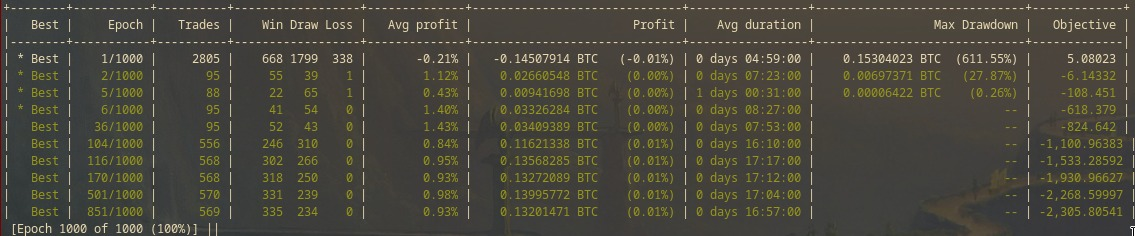
\includegraphics[width=\linewidth]{Imagens/freqtrade2.jpeg}
  \legend{Optimization application running. Resource: The authors.}
\end{figure}
% \clearpage
\begin{figure}[ht]
  \centering
    \caption{\label{fig:freqtrade-running} Optimized Strategy Suggestion}
  % \caption{\label{fig:diagrama-freqtrade} Diagrama esquemático simplificado -
  %   comunicação cliente-servidor}
  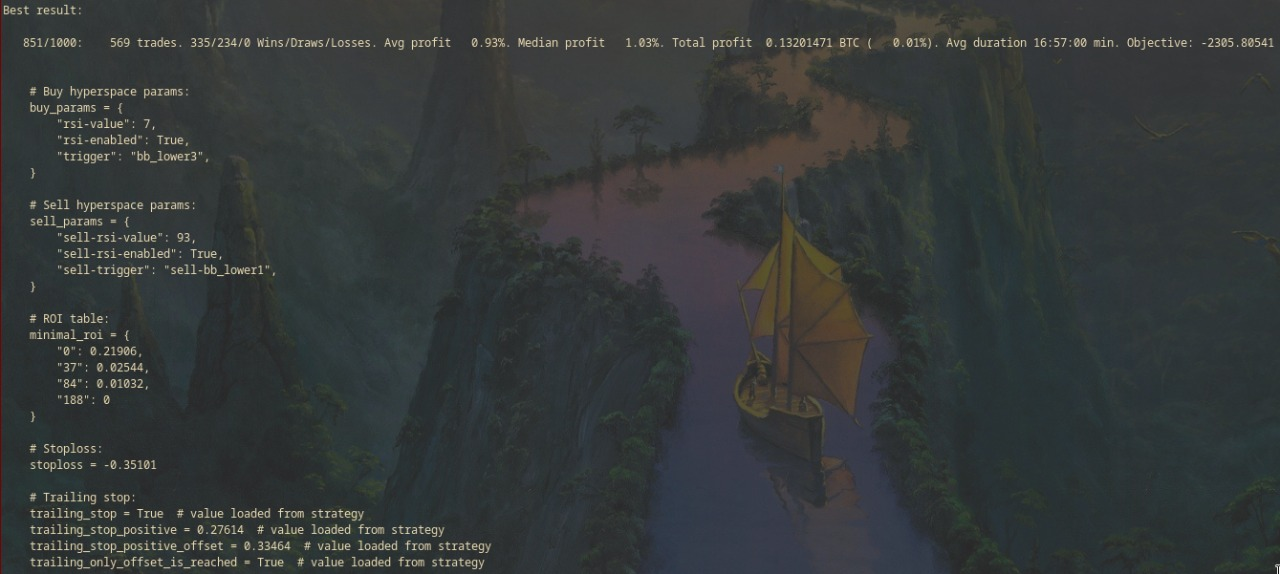
\includegraphics[width=\linewidth]{Imagens/freqtrade3.jpeg}
  \legend{Output to be placed under the strategy file. Resource: The authors.}
\end{figure}

By configuring the file,
\begin{shell}
cd studious-carnival/user_data/config.json
\end{shell}

We can hook the application to our Telegram account and our exchange. For example, one of the options of exchange is Binance \footnote{The markdown ``<<>>'' symbolizes that is a key you would need to provide}.

\begin{python}
"exchange": {
        "name": "binance",
        "key": "<<public-key>>",
        "secret": "<<secret-key>>",
        "ccxt_config": {"enableRateLimit": true},
        "ccxt_async_config": {
            "enableRateLimit": true,
            "rateLimit": 200
        },
\end{python}

And, the Telegram configuration can be configured as,

\begin{python}
"telegram": {
        "enabled": true,
        "token": "<<token>>",
        "chat_id": "1272433706"
      },
\end{python}

% \clearpage

Also, it's possible to test our strategy on past data. We have to call the ``backtesting'' command to that end.

\begin{shell}
sudo docker-compose run --rm freqtrade backtesting --strategy bbrsi6 --timeframe 1h
\end{shell}

\begin{figure}[ht]
  \centering
    \caption{\label{fig:freqtrade-running} Output backtesting history}
  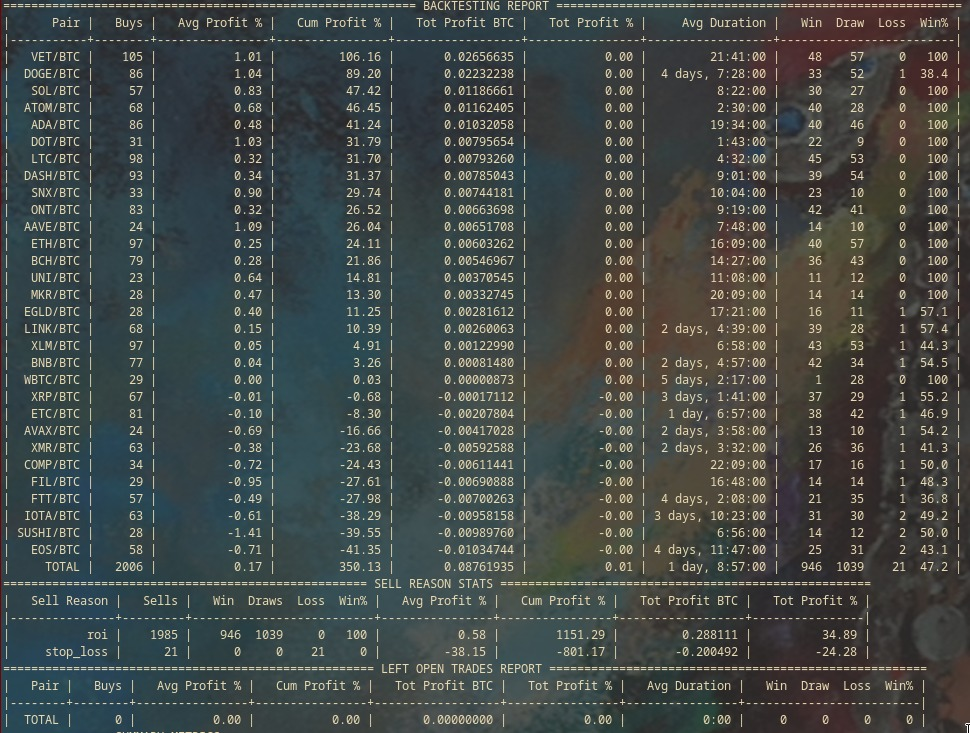
\includegraphics[width=\linewidth]{Imagens/freqtrade4.jpeg}
  \legend{Performance per crypto-coin pair. Resource: The authors.}
\end{figure}

\begin{figure}[ht]
  \centering
    \caption{\label{fig:freqtrade-running} Summary about the backtesting performance}
  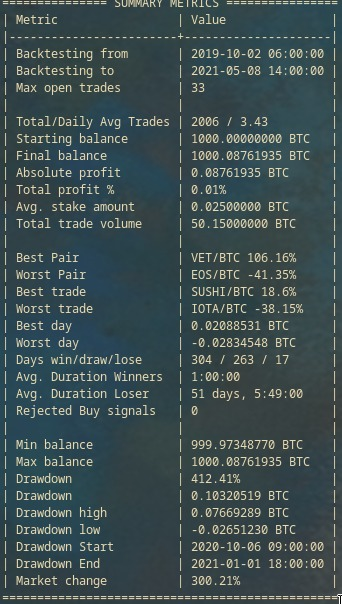
\includegraphics[width=0.3\linewidth]{Imagens/freqtrade5.jpeg}
  \legend{Major information. Resource: The authors.}
\end{figure}

Finally, our application can be run in dry-mode (real-time simulation) \footnote{also configured under config.json}, or with real money.

\begin{python}
"dry_run": false,
\end{python}

Launch the application in the shell, with the following command.
\begin{shell}
sudo docker-compose run --rm freqtrade trade -s bbrsi6 -c user_data/config.json
\end{shell}

\begin{figure}[ht]
  \centering
    \caption{\label{fig:freqtrade-running} Telegram Interaction, application running}
    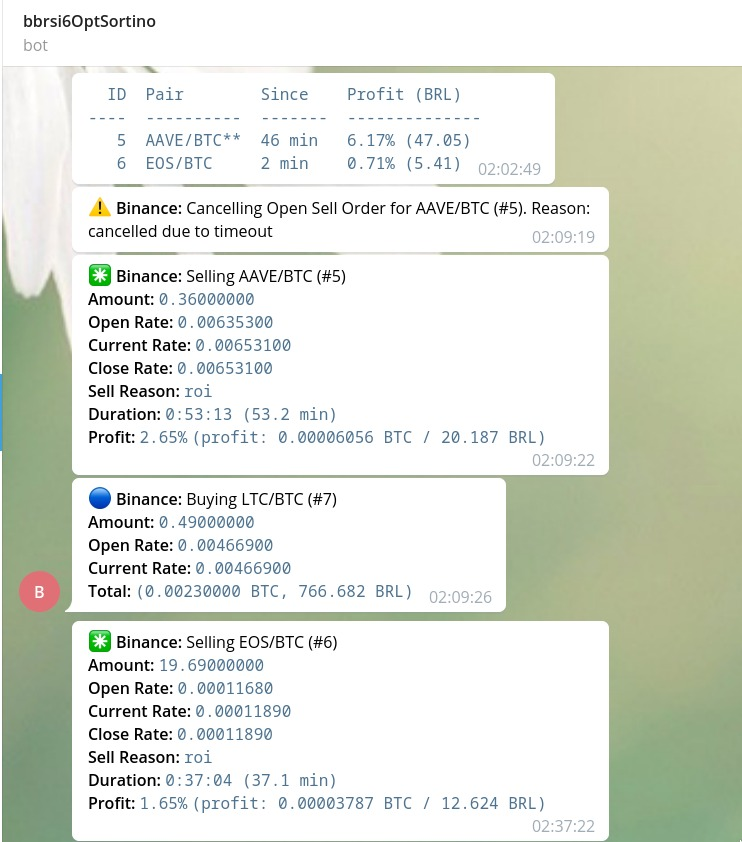
\includegraphics[width=0.45\linewidth]{Imagens/freqtrade1.jpeg}
  \legend{We can monitor and control the application through telegram. Resource: The authors.}
\end{figure}

\subsection{Academia Applications}
\label{subsec:res-academia}

We opted to work with applications written in Python, Julia and
Clojure(Script). Because, the student already is familiar to these
languages. In fact, many of the applications brought in this work has
been cuts of real problems the authors faced in Academia. These
simulations are thus a deepening of how these solutions emerge.
% Optou-se a estudar aplicações escritas em Python, Julia,
% Clojure(script). Pois, o autor possui histórico de
% utilização dessas ferramentas. Com efeito, a pesquisa constituiu, em
% grande parte, na junção de todos os esparços projetos em que o autor
% já havia colaborado ou desenvolvido. E, no aprofundamento da
% compreensão de todas esses projetos, para que fosse possível fazer uma
% apresentação coesa do ferramental utilizado.

\subsubsection{DifferentialEquations.jl}
Julia has been invented to work with scientific computation. The
optimized computation of Julia compares to FORTRAN and C++. Thus, we
chose to use a totally julia-written package, called
\textit{DifferentialEquations.jl}. This package can be used to solve a wide
range of differential equations.

\paragraph{Rumor Propagation Model}

Piqueira \cite{piqueira2010rumor} proposed a model based on Daley-Kendal \cite{daley1964epidemics} for rumor propagation\footnote{There are many other versions considering some kind of variation. In another modern paper, Piqueira consider fact-checkers \cite{piqueira2020daley}} as, 

\begin{equation}
  \begin{align*}
    \dot{I} &= − \beta k SI \\
    \dot{S} &= \beta kSI - \alpha kS (S+R)\\
    \dot{R} &= \alpha k S(S+R)
  \end{align*}
\end{equation}


\begin{figure}[ht]
  \centering
    \caption{\label{fig:diffeq-case1} Rumor Propagation Model - Hard information}
    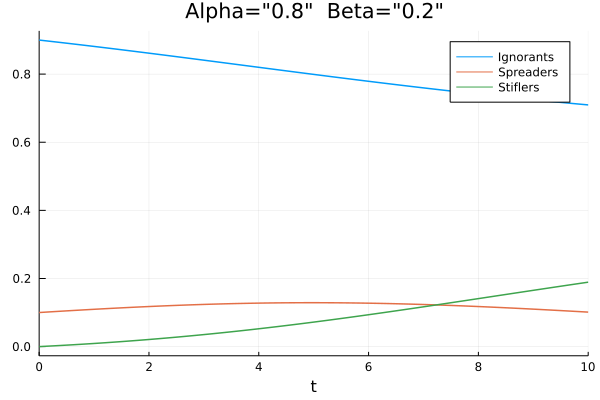
\includegraphics[width=0.5\linewidth]{Imagens/fig09.png}
  \legend{$\alpha = 0.8$ and $\beta=0.2$. Resource: The authors.}
\end{figure}

And, we could easily use Julia and it's package to investigate the behavior of these equations. By reading the paper, we understand $\alpha$ means how hard an information is hard to get, learn or remember etc. At the same time, $\beta$ has to do with how much an information is attractive, scarce (meaning unique), socially relevant etc. And, $k$ has to do with normalization of the $\alpha, \beta{} \, \textrm{and the total population}$. if $\alpha + \beta = 1$ then we can set $k=1$, simplifying the equations.%


We then can then experiment and derive conclusions, for an example, that extremely important information which is also hard to get will have a limiting rate of Ignorants and people who contain that information, but do not propagate it (Stiflers). At the same time, spreaders will have an oscillating response, just as to maintain the limiting rate of ``knowers'' (\autored{fig:diffeq-case1}).

\begin{figure}[!htb]
  \centering
    \caption{\label{fig:diffeq-case2} Rumor Propagation Model - Effects on Spreaders}
    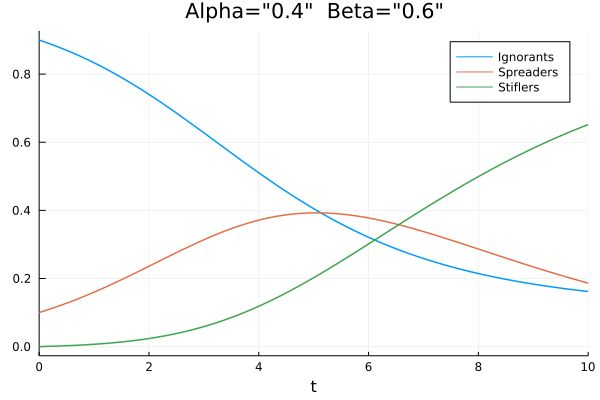
\includegraphics[width=0.5\linewidth]{Imagens/fig95.png}
  \legend{$\alpha = 0.4$ and $\beta=0.6$. Resource: The authors.}
\end{figure}

At the same time, we can learn about the counter-intuitive effect of making a relevant information, with good spreading changes, too accessible. That can make part of the public unaware of it. Because the Spreaders may lose interest in talking about it, due to too many people talking about it. And, then, all of the sudden, these Spreaders become Stiflers who forgot or do not talk about the subject anymore for whatever reason (\autoref{fig:diffeq-case2}).
\clearpage
\subsubsection{Teaching abstract concepts}

Some animations in Clojure can be done using a great deal of
libraries. And, some of them can be used for understanding STEM
related abstractions.

\paragraph{Cellular Automata}

Proposed by Wolfram \cite{wolfram1983cellular}, a useful way to
understand and contemplate complexity can be by visualizing cellular
automata. From these seemingly simple rules arise immense complexity (\autoref{fig:ca1}).

\begin{figure}[ht]
  \centering
    \caption{\label{fig:ca1} Cellular Automata with Clojure}
  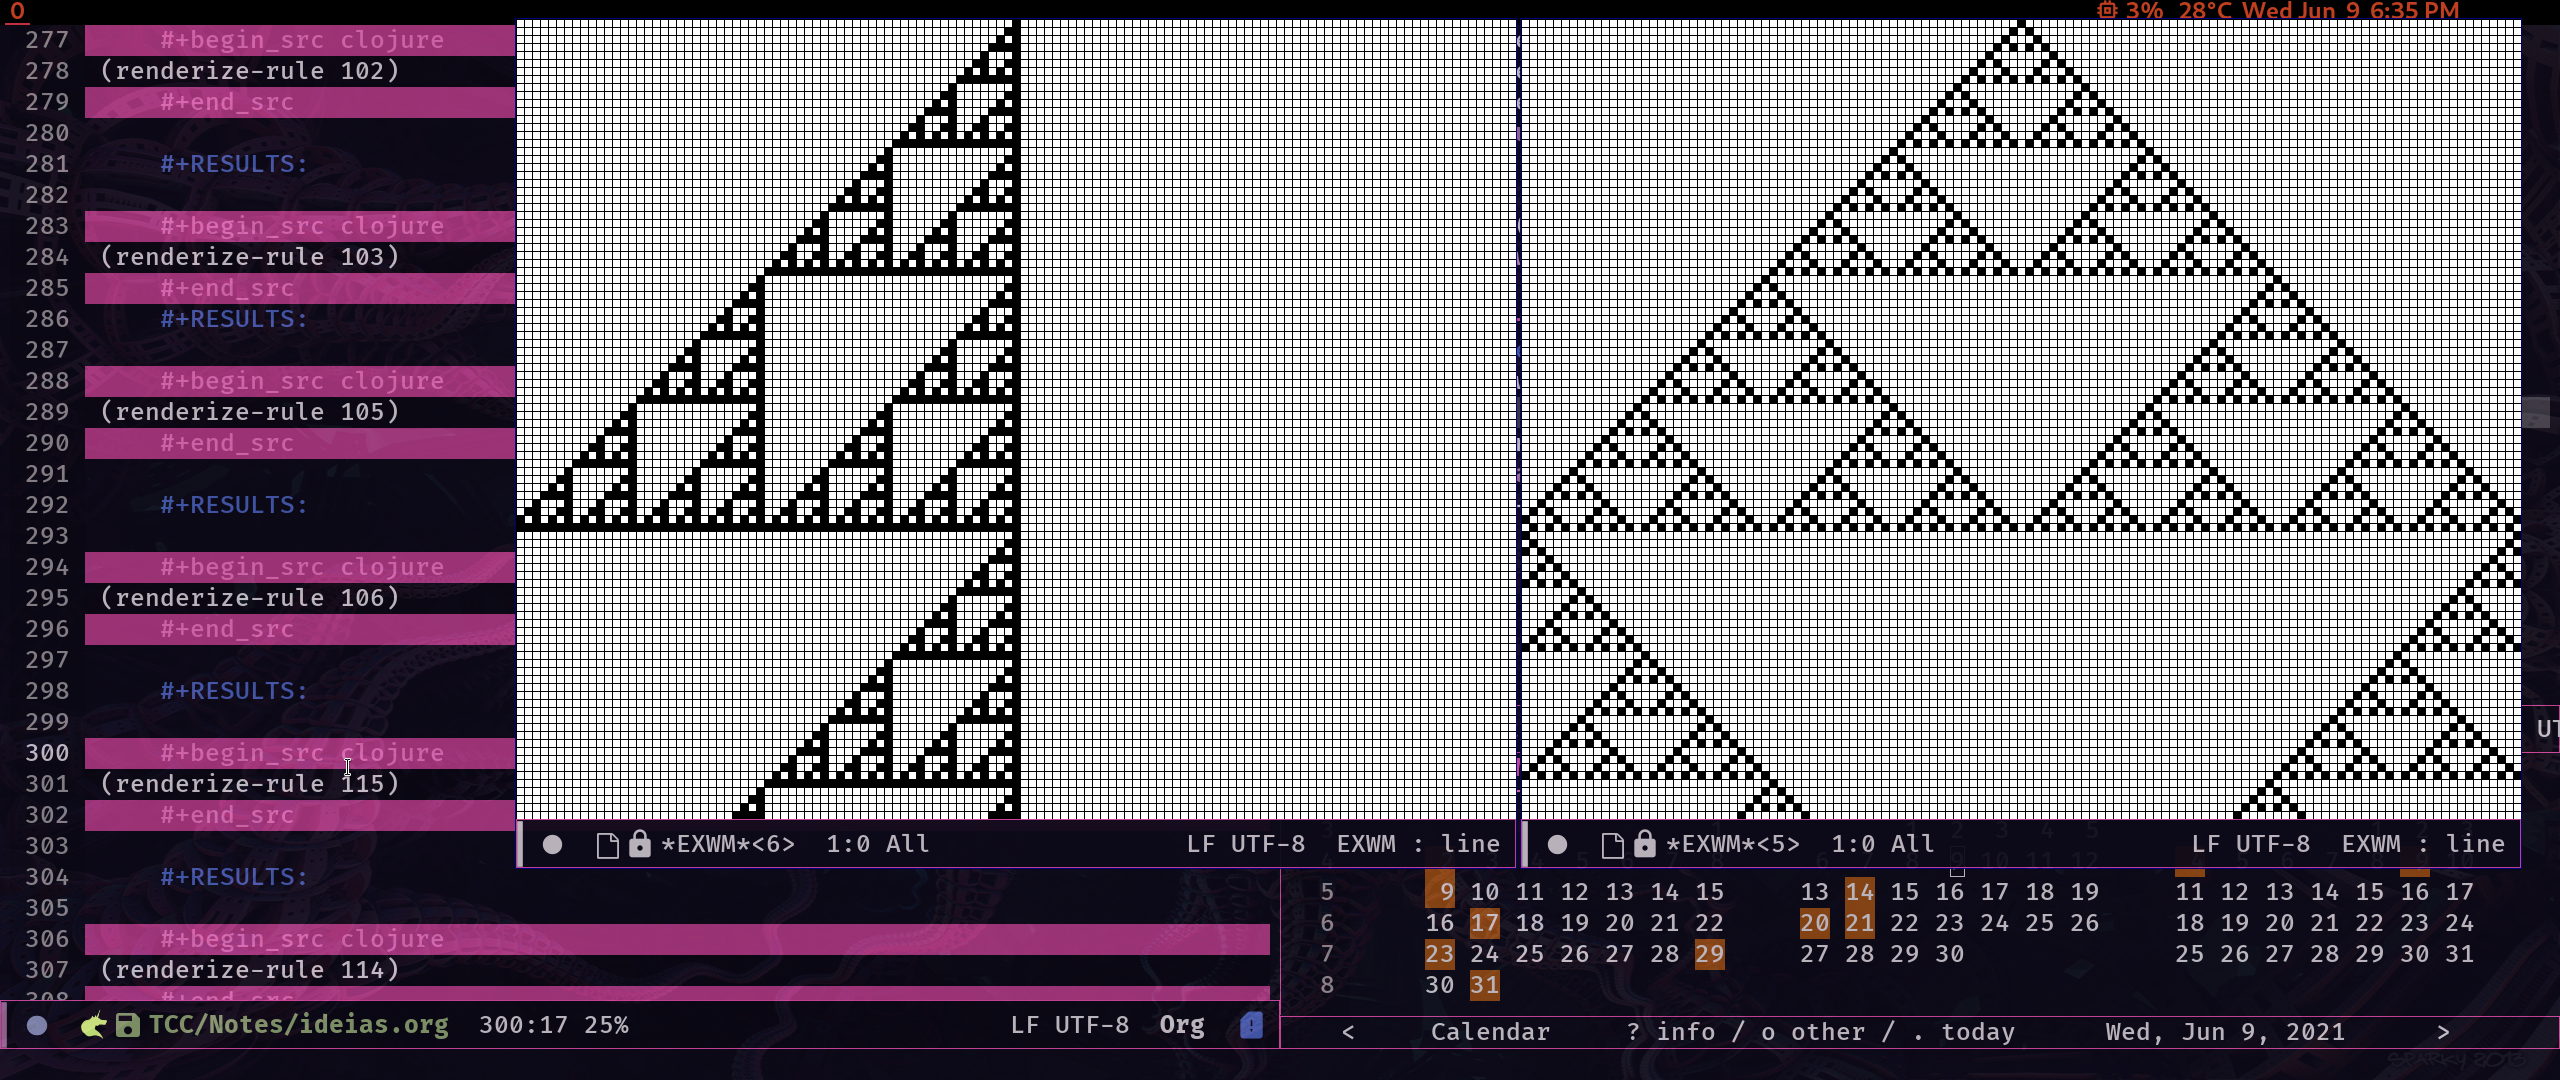
\includegraphics[width=0.7\linewidth]{Imagens/CA/ca1.png}
  \legend{Simulating simple rules, arising complexity. Resource: The authors.}
\end{figure}

\paragraph{Electromagnetism}

In Clojure2D library, we can write waves that imitate electromagnetic
waves behavior (\autoref{fig:em}). 

\begin{figure}[ht]
  \centering
    \caption{\label{fig:em} Electromagnetism with Clojure}
  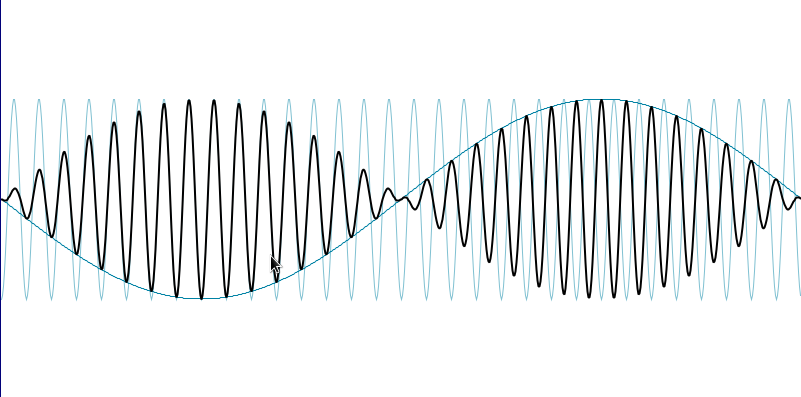
\includegraphics[width=0.7\linewidth]{Imagens/CA/eletromag-is.png}
  \legend{Resource: The authors.}
\end{figure}

\paragraph{Calculus}

Pre-calculus knowledge of how $sin(\theta)$ behaves. Probably, explain
rates of variation and other concepts with interactive
simulations. The student would be able to actively engaged, manipulating the
code, angular rate etc (\autoreg{fig:calc}).

\begin{figure}[ht]
  \centering
    \caption{\label{fig:calc} Calculus and rates of changes}
  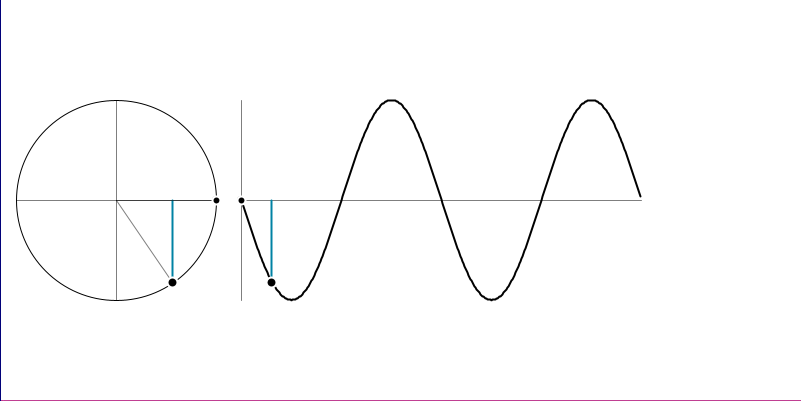
\includegraphics[width=0.7\linewidth]{Imagens/CA/calc1-is.png}
  \legend{Resource: The authors.}
\end{figure}

\paragraph{Analytical Geometry}

With Clojure2D there are implemented simulations of vector projection
simulation. These could be used in teaching analytical geometry (\autoref{fig:ga}).

\begin{figure}[ht]
  \centering
    \caption{\label{fig:ga} Vector projection simulation}
  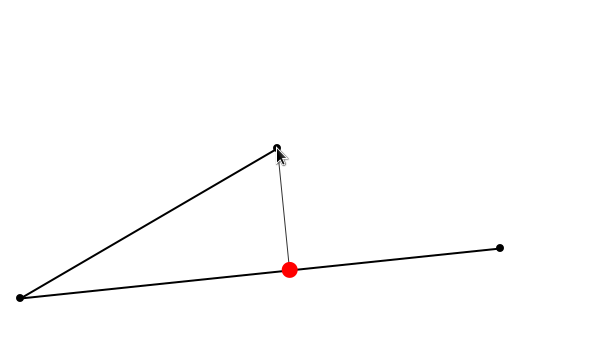
\includegraphics[width=0.7\linewidth]{Imagens/CA/GA-is.png}
  \legend{Resource: The authors.}
\end{figure}

\paragraph{Fluid Viscosity}
Also, one could use implemented simulations of free fall bodies
changing of medium. These models show how a body changes motion
under such changes (\autoref{fig:vis}). 

\begin{figure}[ht]
  \centering
    \caption{\label{fig:vis} Body under gravity - Viscosity}
  
\includegraphics[width=0.7\linewidth]{Imagens/CA/fv-is.png}
  \legend{Resource: The authors.}
\end{figure}

% \subsection{A intersecção}

% Com Clojure(Script), Bash e \LaTeX{}, foi possível criar tanto
% simulações que estendem a compreensão de fenômenos físicos do campo
% abstrato ao visual. Também, empregou-se de Closh e Babashka, duas
% bibliotecas de Clojure dedicadas a interoperabilidade com Bash, a qual
% se processava milhares de arquivos, por meio de pipelines de
% arquitetura complexas. Assim, facilitando a escrita de uma quantidade
% enorme de relatórios técnicos na área de segurança do trabalho. 

% Quanto a Clojure(Script), foram pesquisadas simulações gráficas, as
% quais inerentemente são simples de se programar em Clojure. Pois, seu
% ecossistema pode interoperar entre JVM (Java Virtual Machine) e
% JavaScript. Assim, dado que ambos Java e JavaScript foram as línguas
% mais populares por décadas, existem uma enorme quantidade de ambientes
% e bibliotecas a nossa disposição. Bem como, Clojure é uma Lisp - e,
% caracteristicamente, essa família é utilizada para prototipagem, vide
% AutoCAD escrito em AutoLisp.

% Dado que existem bibliotecas dedicadas a Mecânica Clássica em nível de
% mestrado, bem como exite capacidades de se renderizar conceitos
% físicos abstratos. Então, decorreu-se a computação de programas que
% demonstravam conceitos de Física, Cálculo, e Computação Generativa.


% Os programas em Julia possuiam cunho numérico. Pois, sua computação
% optimizada compara-se a performance de FORTRAN e C++. Assim, o
% principal pacote estudado foi DifferentialEquations.jl, a qual pode
% ser utilizada para resolver uma gama de equações diferenciais,
% incluindo a categoria Estocástica.

% O programa em Python é de processamento de imagens. Escolheu-se essa
% aplicação, pois demonstra o quão abrangente é a portibilidade de
% programas escritos em outras línguas ao Python - principalmente,
% devido a grande comunidade de cientistas e programadores que o
% utilizam.



% \section{Organização cronológica}
\section{Chronological Organization}

The present work has been manager through Gantt
diagrams\footnote{Using \LaTeX}. Also, we used dynamic agendas builtin
in Emacs. Thus all visual framing of time has been done by either one
these two.

\begin{figure}[ht]
  \centering
  \caption{\label{fig:calendar} Emacs's Calendar}
  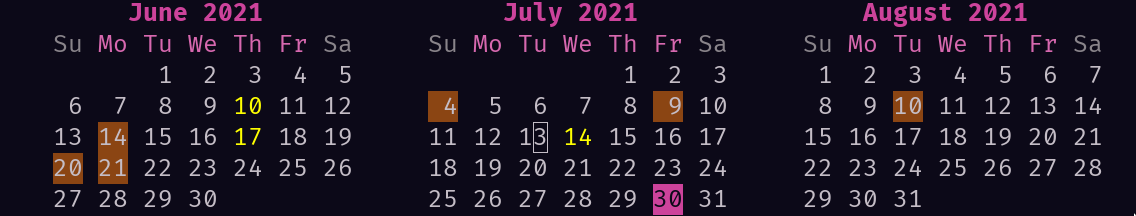
\includegraphics[width=0.7\linewidth]{Imagens/calendar.png}
  \legend{Schedules, deadlines and vacations marked. Resource: The authors.}
\end{figure}

\begin{figure}[ht]
  \centering
  \caption{\label{fig:gantt} Gantt Chart produced with latex}
  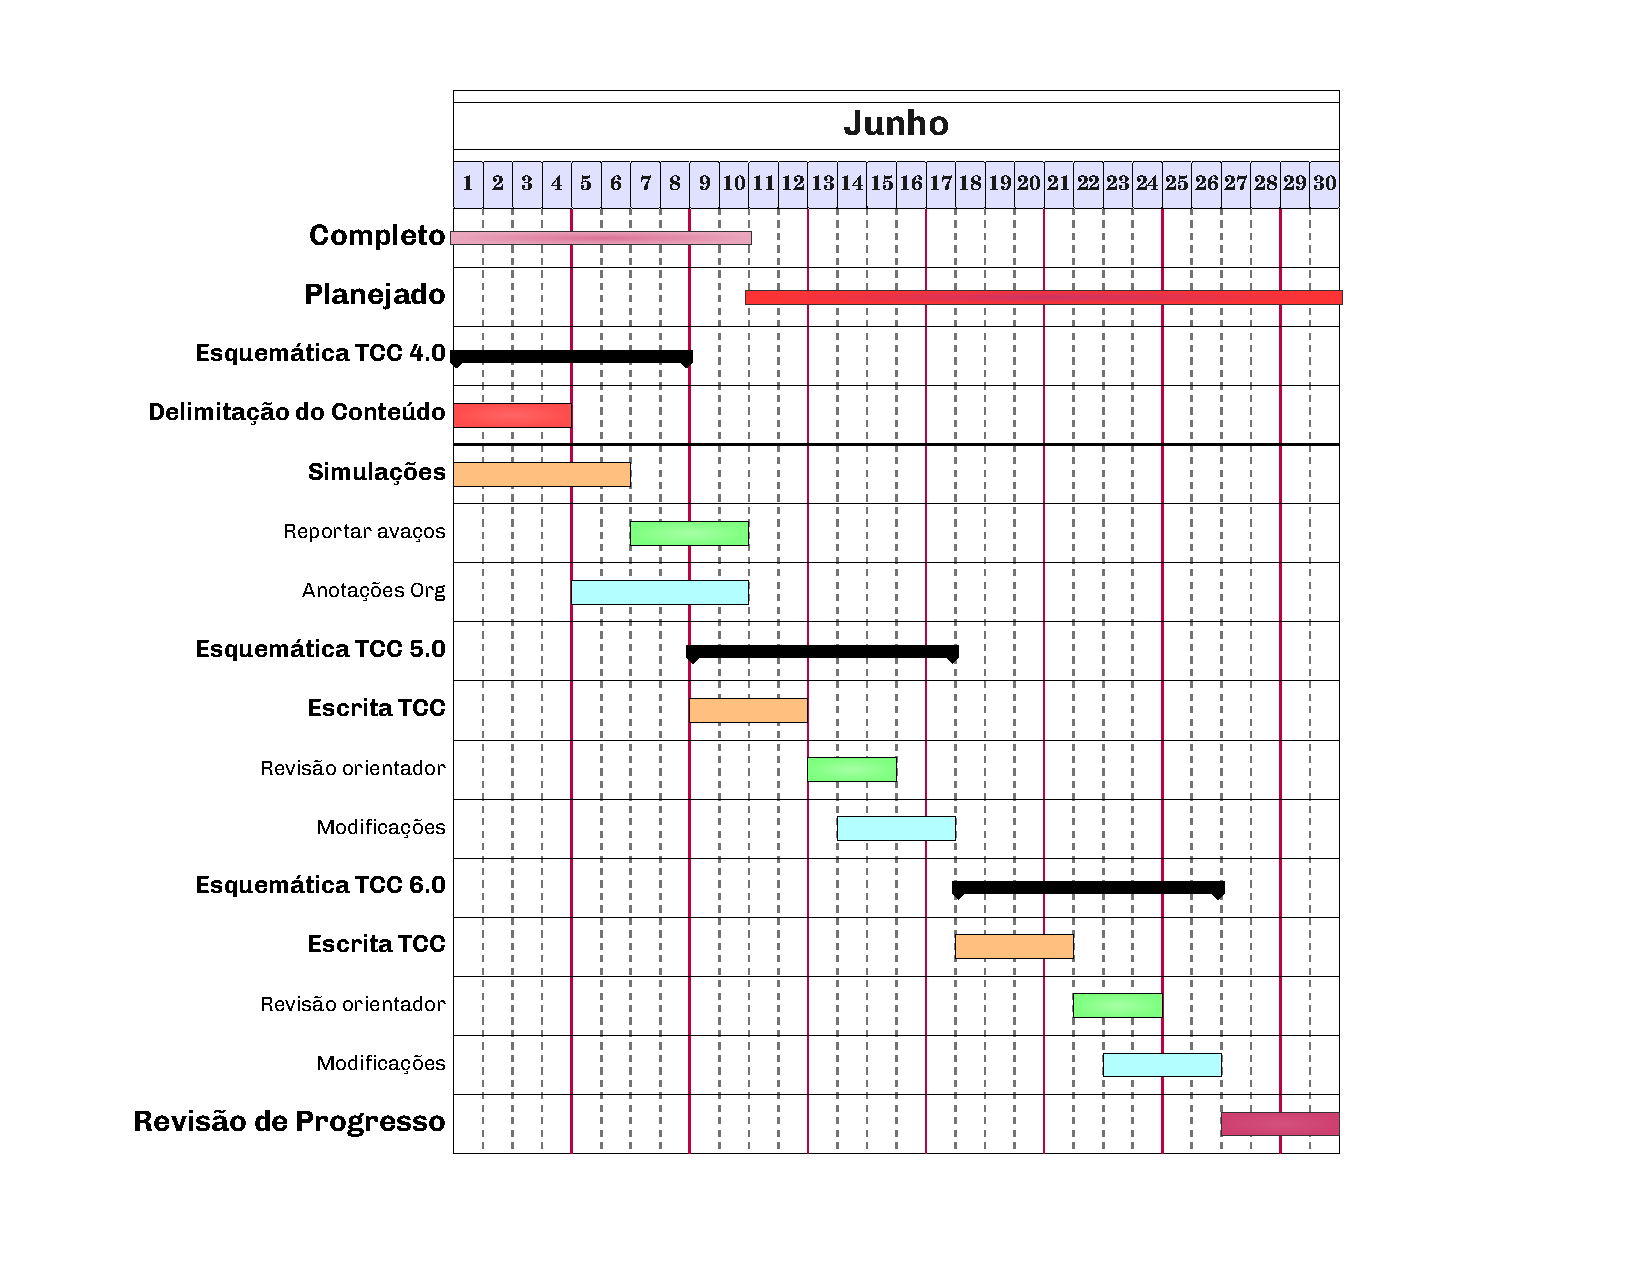
\includegraphics[width=0.7\linewidth]{Schedule/cronograma-tcc.pdf}
  \legend{Gantt for July. Resource: The authors.}
\end{figure}

% \begin{figure}[ht]
%   \centering
%   \caption{\label{fig:gantt} Gantt Chart produced with latex}
%   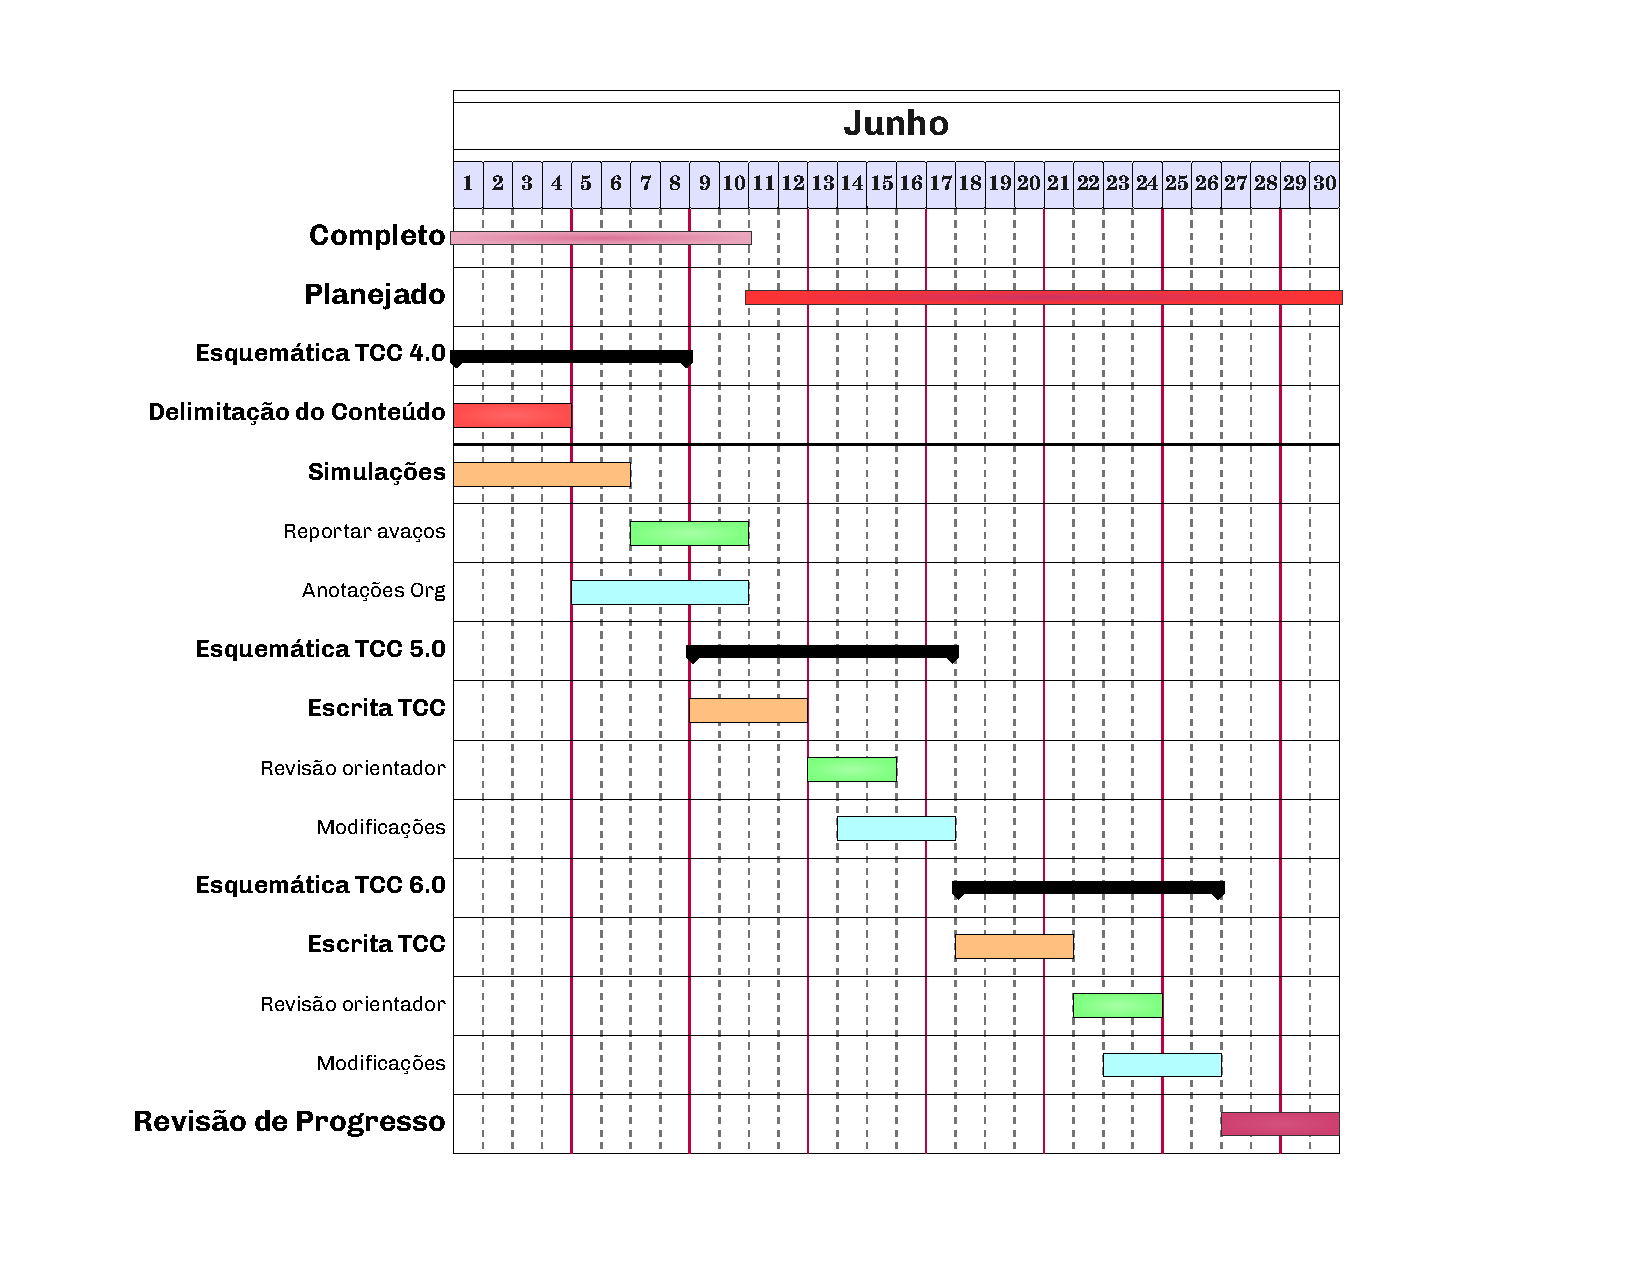
\includegraphics[width=0.7\linewidth]{Schedule/cronograma-tcc.pdf}
%   \legend{Resource: The authors.}
% \end{figure}

\begin{figure}[ht]
  \centering
  \caption{\label{fig:org-pomodoro} Daily Pomodoro timing (Using Org-pomodoro)}
  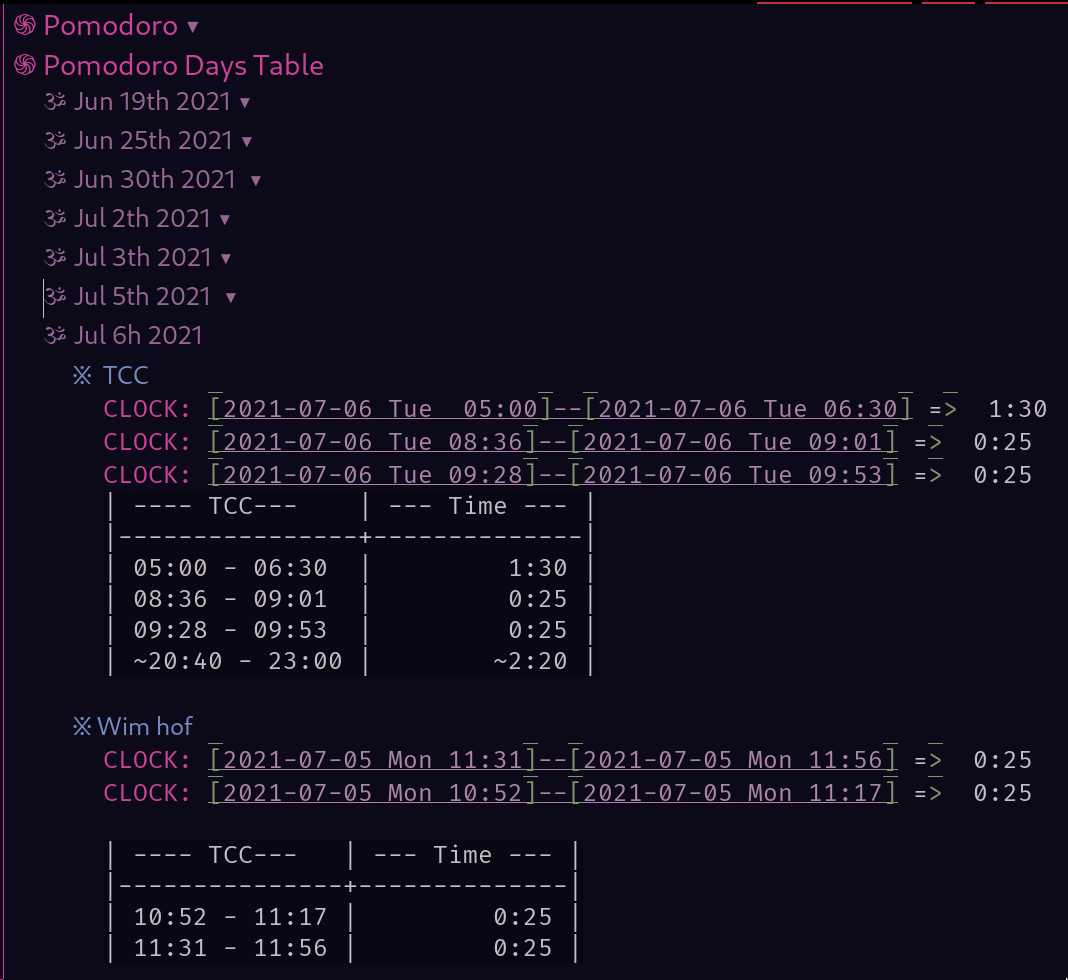
\includegraphics[width=0.4\linewidth]{Imagens/daily-pomodoro.png}
  \legend{Tables written in Metrics.org file. Resource: The authors.}
\end{figure}

\begin{figure}[ht]
  \centering
  \caption{\label{fig:org-agenda} Org-agenda, an Orgmode feature}
  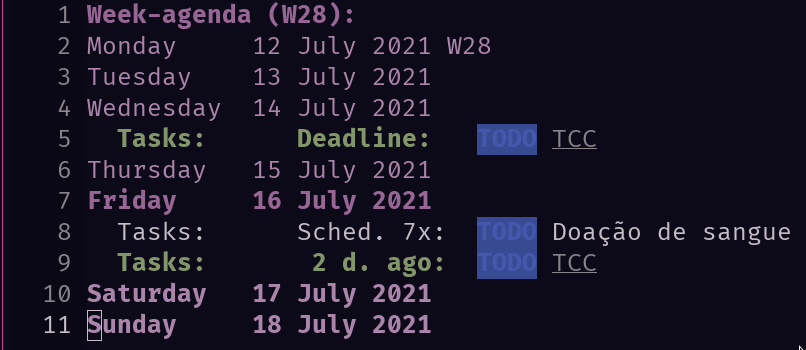
\includegraphics[width=0.7\linewidth]{Imagens/weekly-agenda.png}
  \legend{Resource: The authors.}
\end{figure}

The system TGD (To Get Done) and TODO-NEXT-DONE has been implemented
using Org-mode synchronized with Org-agenda.

% A organização do projeto se deu utilizando os diagramas de Gantt, e as
% agendas dinâmicas, /org-agenda/, nativas do Emacs. Por conseguinte,
% toda a comunicação sobre o projeto foi materializado por meio de
% cronogramas e agendas.

% \section{As fases da escrita da Monografia}
% Iniciou-se a escrita da monografia pela pesquisa bibliográfica, dado
% que a pesquisa se categoriza, epistemologicamente, como uma Análise
% Exploratória. O \textit{template} utilizado para escrita do projeto
% foi o \abnTeX{}, biblioteca do \LaTeX dedicado a escrita de documentos sob as normas ABNT.

\section{Note collection and ABNTeX2}

The \textit{org-mode} organizational toolkit has been developed in such a way
that reproducible research is the default
\cite{stanisic2015effective}\footnote{On a similar note, watch the
  video entitled
  ``\href{https://www.youtube.com/watch?v=AP4LX8L7MFM}{Reproducible
    Research with GNU Emacs and Org-mode} by Thibault Lestang (University of Oxford)''}.
% O \textbf{org-mode} é uma ferramenta de organização e anotação, desenvolvida
% para pesquisa e reprodutibilidade de pesquisas. Assim, todas as etapas
% de desenvolvimento do projeto foram desenvolvidas e documentas utilizando
% essa ferramenta.
\begin{figure}[ht]
  \centering
    \caption{\label{fig:literate-programming} Literate programming in Org-mode}
    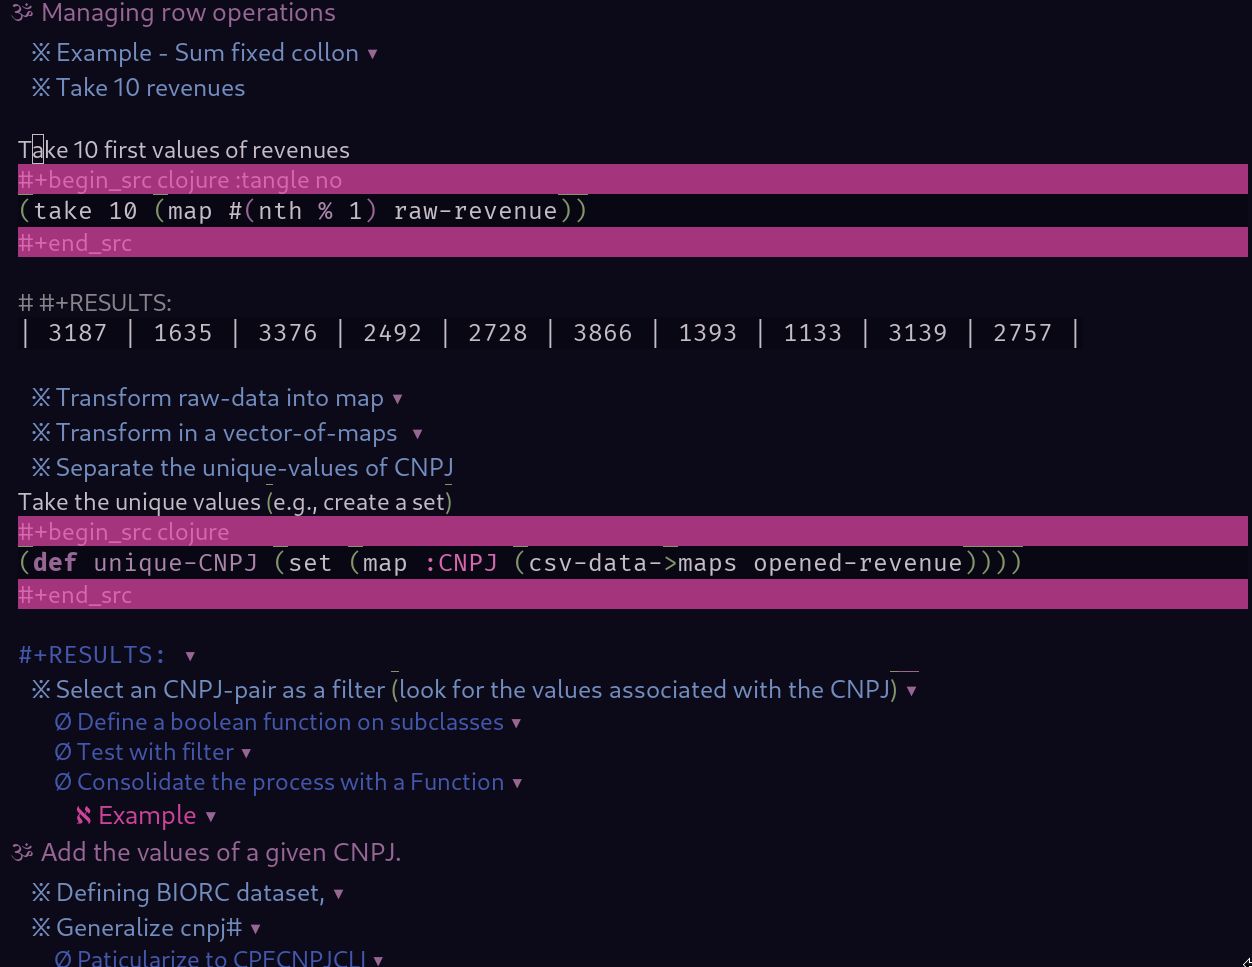
\includegraphics[width=0.7\linewidth]{Imagens/org-mode.png}
  \legend{Mixing text, code and evaluation. Resource: The authors.}
\end{figure}

Org-mode enables \textit{Literate Programming}\footnote{conceptualized
by Donald Knuth\cite{knuth1984literate}, and has been commonly adopted
by design or naturally arose in GNU/Emacs, Org-mode and \LaTeX{}.}, which is mixing code
and notes - not meant to be read by an interpreter/compiler. It's even
possible to evaluate code inside Orgfiles. So, by reconstructing my
earlier works in a orderly manner, this document was possible.
% A documentação implícita ao desenvolvimento é uma
% característica fundamental e pensada do Org-mode. Pois, segue o
% paradigma de \textit{Literate Programming}. Assim, há uma mistura de
% notas e códigos em um mesmo ambiente. Fazendo que a prototipação do
% código seja automaticamente documentável.

Converting .org files to .tex and thus .pdf files is as
simple as calling a function in Emacs \footnote{Calling a function in
  Emacs takes one to five key-strokes
depending on how you call it.}. Emacs itself has been called a
self-documenting system\footnote{https://www.emacswiki.org/emacs/SelfDocumentation}. And, truly, if one wishes, all documentation
of Emacs is contained inside the help-system in pure-text format. To
learn a certain thing about Emacs, one would never have to leave it's
environment.

Finally, translating the main .tex output into ABNT norms consisted in
utilizing the canonical features of the ``abntex2'' class document.

\begin{figure}[ht]
  \centering
  % \caption{\label{fig:tower} Esquemática de uma torre de interpretadores}
  \caption{\label{fig:abntex} ABNT specification class in LaTeX}
  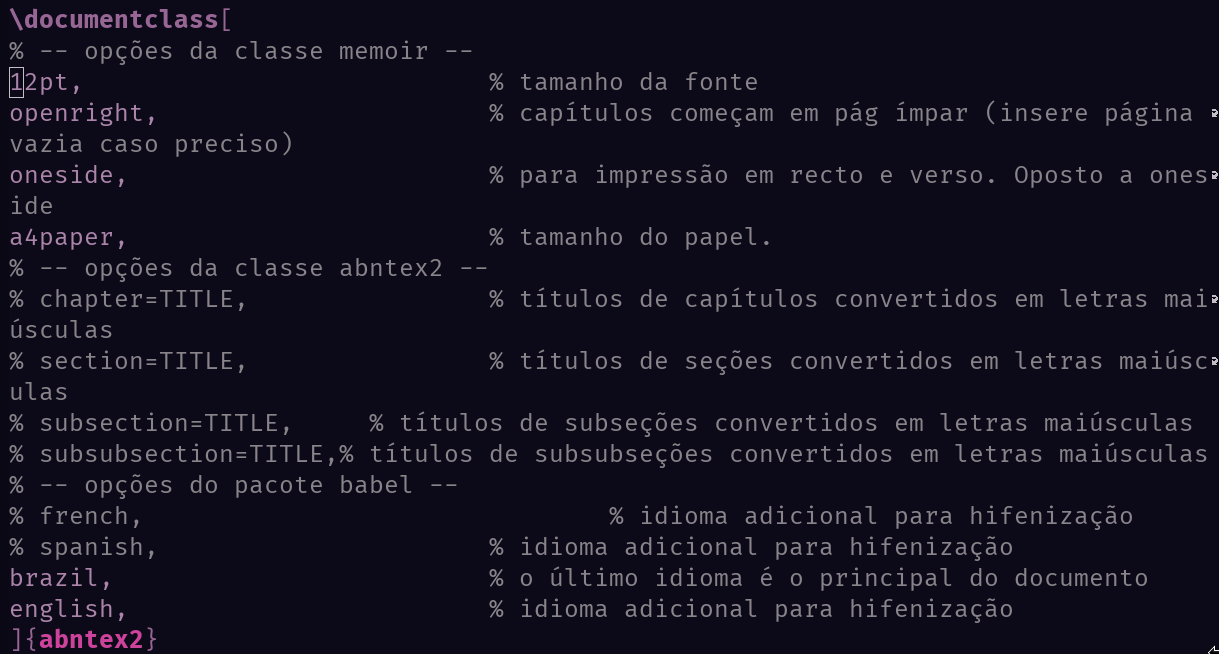
\includegraphics[width=\linewidth]{abnt.png}
  \legend{Source: the authors.}
\end{figure}

The cover and typographical details were constrained to the particular
style prescribed by the Engineering School of Lorena - University of
São Paulo (EEL-USP).

\section{Bibliographical Research}
% \section{Pesquisa bibliográfica}

The bibliographical research was done majorly through sites, when
dealing with historical data on programming or programs
itself. Because these kinds of data are self-documented by the open
community.

In turn, when speaking about theoretical ideas or
benchmarks, the research was done by DuckDuckGo, ACM, Google
Scholar or ArXiv\footnote{Currently(2021) contains 1.9mi. papers
  openly available}. The format found were mostly articles of books in
these researches.
% A pesquisa bibliográfica foi em grande parte encontrada em sites sem
% autores. Pois, a documentação foi criada ou pela comunidade, ou por
% instituições, não unicamente publicada em formato de livro ou artigo.

Vast literature was found on Julia's
DifferentialEquations.jl. Due to the fact that the Julia community
arose from Academia (MIT), and it's main goal in applied research.
% Da parte acadêmica, como o pacote de resolução de equações
% diferenciais, em Júlia, encontrou-se vasta literatura. Até porque, a
% língua foi criada para resolver problemas computacionais tocantes
% principalmente a comunidade científica do MIT.

Finally, some documentation was found only through GitHub, as OR-Tools
and Clojure's Clojure2D library. These were entirely electronic publications.
% Por fim, algumas ferramentas apenas existem documentadas e contidas
% inteiramente em repositórios, como o Github. Foram os casos do
% OR-Tools e as simulações em Clojure. São publicações puramente eletrônicas.

% \section{Revisão contínua}

% Dentro do cronograma concebido para desenvolvimento da monografia,
% pôs-se metas e etapas de escrita do documento. E, estipulou-se os
% conteúdos necessários para cada nova versão do documento, aliado a uma
% data limite. Assim, o retorno do orientador ao orientado pode se dar
% mais frequentemente.

% \section{Organização da apresentação}

% Como se está utilizando de diversas ferramentas e extensões dentro do
% Emacs e do Org-mode, em particular, optou-se por utilizar uma de suas
% funcionalidades dedicada a apresentações. 

\chapter{Conclusion}
% \chapter{Conclusão}
Among the open source initiatives, there exist virtually an
application for any one given field one may pick. That is, current
research is mostly done using some kind of software application. Even
more, Art, Organization, and Humanities also benefit from computation,
not only Science, Technology, Engineering and Math (STEM) areas.
% Dentro das iniciativas Open Sourced, existem virtualmente aplicações
% para todas as áreas das aventuras do ser humano. Isto é, seja o uso de
% computação gráfica, processamento de imagens, expressões artísticas,
% ou ferramentas de organização, há um software escrito para esse fim.

These open software almost majorly have State of the Art research on
Computation backing them. Although the common belief may be that close
software development has the upper-hand on quality and support, that
is not the case.

One of the motives may be giving to the copy-left
licenses coercing users of pieces of it's application to publish their
software under the same license. Or, one may argue that once a person
is involved in the Open Community and benefits from free and quality
support from other user-developers or project maintainers. Then,
nothing is more fair than contributing, when he adds to the pile of
data and knowledge which boosted his way forward. Thus, the community
achieves grow and continuity.
% É observável a falta de competição quanto a quantidade e qualidade de
% softwares fechados e abertos. Ademais, a capacidade de
% extensão dos softwares livres, por meio das quatro fundamentais
% liberdades de suas licenças, permitem que exista uma variedade imensa
% de uso de uma mesma ferramenta. Por fim, o enriquecimento dessa
% participação colaborativa solidifica e generaliza as ferramentas
% abertas - num grau e rapidez inimagináveis, comparados ao processo de
% desenvolvimento por uma equipe fechada.

We have demonstrated many different uses of open software, with no
closed sourced, paid, software. These were both in the sector of
Industry and Academia applications. OR-Tools, FreqTrade, DifferentialEquations.jl and Clojure2D library developed majorly by the community use State of the Art mathematical and computing tools. OR-Tools has been, for an example, the champion in three categories of MiniZinc Challenge in 2020\footnote{https://www.minizinc.org/challenge2020/results2020.html}.
% Demonstrou-se diversos usos desses software, sem paralelos, na
% Indústria e na Academia. Ambos possuem algorítimos na fronteira da
% ciência, a qual o uso apenas é limitado pela imaginação e capacidade
% formativa do usuário-desenvolvedor. Assim, é imprescindível que no
% curso de engenharia se tenha uma ampla formação com base nos softwares
% livres, sob os quais a computação moderna subiste.

We also pointed some entry doors to the use of FOSS-based systems. We
discussed why to use the Kernel Linux, and the GNU applications which
permeates GNU/Linux system's functionalities. Furthermore, we demonstrated
the benefits of inserting oneself in the social community around these
open sourced initiatives et al. Finally, the effectiveness and
plausibility of an running under a entirely FOSS-based system -
GNU/Linux with EXWM - has used to produce this work. 
% Apontou-se algumas portas de entrada, fundamentais, a esse paradigma,
% os sistemas com Kernel Linux, as aplicações GNU as quais lhe dão
% roupagem, e por fim os sistemas sociais onde se desenvolve os
% softwares, como a plataforma de versionamento Git/Github. Ademais,
% demonstrou-se, com efetividade, que é possível construir e rodas todas
% essas aplicações num sistema totalmente aberto.

\bibliography{bib}

\end{document}
